\chapter{Introduction}



\section{Motivation} \label{sec:Einl:Motivation}
The Finite Element Method (FEM) is a numerical technique for finding approximate solutions to boundary value problems for partial differential equations. FEM contains linear FEM and non-linear FEM. 
Linear analysis follows the equation $K\cdot D = F$, in which $K$ stands for stiffness matrix, $D$ stands for  displacement, and $F$ stands for force. It means that the correlation of force and displacement is linear. This relation between force and displacement is only valid for materials that have elastic linear property. But in real situation, elastic materials such as steel has also non- linear region. (see the Figure \ref{fig: nonlinear}). The property of steel is elastic linear up until yield point. Then the steel is yielding and becomes non-linear. Non-linear states include geometry non-linear and material non-linear. The example in Figure \ref{fig: nonlinear} describes a non-linear case and it also the main topic of this thesis. In the fields of engineering and science, FEM is a powerful tool in producing strength visualization and can help engineers to minimize weight, materials and costs. The accuracy of solution are only limited by the quality of model and by the available computational power.  Ever since the computational power has been improved enormously, the FEM software has offered a wide range of simulations of complex model designs and system analyses.  \newline
AMfe is a nonlinear finite element code for structural application at the chair of applied mechanics in Technical University of Munich. AMfe Toolbox is developed in Python and Fortran. Python is a high-level, interpreted, and dynamically-typed programming language.  There are many numerical packages built on Python, such as Numpy, Scipy, Pandas. These packages provide high-performance and easy to use data structures, both of which match the FEM developing work. The fact that Python is a high-level programming language makes it less time-consuming to develop the code. However, Python is slow for repeated execution of low-level task. Each Python operation comes with a small type-checking overhead, and when many repeated small operations add up, the overhead becomes significant. For this reason, A part of the AMfe code is rewritten in Fortran. Fortran is a general-purpose and imperative programming language that is specially tailored for numeric computation and scientific computing. Therefore, the combination of Python and Fortran retains the advantages of both - the easy-to-develop nature of Python and the fast numeric computation in Fortran. The aim of AMfe Toolbox is to solve and analyse FEM problems, especially structural mechanical problems.
The toolbox contains several modules with different functions to solve problems step by step. A simple structure of AMfe is depicted in Figure \ref{fig: Overview2}. Displacement, stress, and strain are three important factors in structural mechanical engineering. The function for calculating nodal displacements is completed in AMfe Toolbox, but functions for calculating nodal stress and strain remain blank. Strain and stress calculations are important in structural mechanical analysis and geometric design. For this reason, functions for solving of stress and strain will be added to AMfe Toolbox. When strain and stress calculations are completed, the aim of research is then shifted to improving the accuracy of these results. In order to do so, stress recovery is an approach to extrapolate the element solution to nodal solution. The goal is to be as accurate as possible in the computed displacements while keeping the computational effort reasonable. When the most important functions are completed and running well, it is time to check if AMfe Toolbox exports the reasonable results. The results of stress and strain from AMfe Toolbox will be compared with a commercial FEM software - ANSYS. The comparison of each element type will be recorded and discussed. 

\begin{figure}
	\begin{center}
		\includegraphics[width=8cm,clip]{nonlinear.pdf}			
		\caption{Stress-Strain curve for steel} \label{fig: nonlinear}
	\end{center}
\end{figure}

\section{Structure of Study}

\begin{figure}
	\begin{center}
		\includegraphics[width=12cm,clip]{Overview.pdf}			
		\caption{Flow chart of structure} \label{fig: Overview}
	\end{center}
\end{figure}

\begin{figure}
	\begin{center}
		\includegraphics[width=12cm,clip]{Overview2.pdf}			
		\caption{Overview of this essay structure} \label{fig: Overview2}
	\end{center}
\end{figure}

This study can be divided into three parts.  Figure \ref{fig: Overview} shows the structural flow chart in this study. The first part is marked with a green box. The main function for this part is to export the data of a meshed geometry using ANSYS Parametric Design Language(APDL) code and import the data into the AMfe Toolbox. This procedure, which is called Pre-Processing, is the first step in solving a problem in Finite Element Analysis. This step also ensures the analyses from both ANSYS and AMfe Toolbox have the same set of elements and nodes. The processing step comes next, which is marked with a yellow box. AMfe Toolbox has several modules with different functions. These modules combined provides all calculation functions needed for processing. This study is focusing on calculating stress and strain. The last part marked by blue is to check the accuracy of strain and stress using different types of elements.

\chapter{Numerical Aspect for Finite Element Formulation}
\section{Shape Function}
\subsection{Quadrilateral Elements}
The goal of the AMfe Code in the structural mechanical field is to get the approximate solutions to position, displacement, stress, and strain. According to the Finite Element theory of W. A. Wall [\cite{FiniteElement} p.75], the approximation is dependent on the shape function $N$. The standard approach to define the shape functions is choosing them as simple polynomials that are associated to nodes. There are $n$ nodes and $n$ shape functions in one single element. The $i$-th shape function takes the value of 1 at the $i$-th node in reference coordinates, then the $j$-th shape function can be written like this: \\

\begin{center}
	if $j$ = $i$ then $N_j\left(\hat{\xi_i}\right) = 1$ \\
	if $j$ $\neq$ $i$ then $N_j\left(\hat{\xi_i}\right) = 0$
\end{center}



for $i$, $j$ = 1,...,n. \\
In Figure \ref{fig: shape_func}, linear and quadratic shape functions are expressed together with corresponding node positions. When referring to an element with three nodes, as shown in the right of Figure \ref{fig: shape_func}, there are three restrictions for each shape functions:

\begin{figure}
	\begin{center}
		\includegraphics[width=10cm,clip]{shape_func.pdf} 		
		\caption{Linear shape function and quadratic shape function.} \label{fig: shape_func}	
	\end{center}
\end{figure}

\begin{center}
	$N_1\left(\hat{\xi_1} = -1\right) = 1$, $N_1\left(\hat{\xi_2} = 0\right) = 0$, $N_1\left(\hat{\xi_3} = 1\right) = 0$;\\
	$N_2\left(\hat{\xi_1} = -1\right) = 0$, $N_2\left(\hat{\xi_2} = 0\right) = 1$, $N_2\left(\hat{\xi_3} = 1\right) = 0$;\\
	$N_3\left(\hat{\xi_1} = -1\right) = 0$, $N_3\left(\hat{\xi_2} = 0\right) = 0$, $N_3\left(\hat{\xi_3} = 1\right) = 1$
\end{center}
For quadratic polynomial, the shape function has three coefficients, and it can be constructed as follows:
\begin{center}
	$p_{quad}\left(\xi\right) = c_0 + c_1\xi + c_2\xi^2$
\end{center}
According to the work of W. A. Wall [\cite{FiniteElement} p. 75], Lagrange polynomials are a general group of polynomials with the node undermentioned association property: a Lagrange polynomial $l_k^n-1$ of order $n-1$ transits $n$ nodes with coordinates $\bar{\xi^j}\left(j = 1,...,n\right)$ of which the single node $k$ equals one $\left(l_k^{n-1} \left(\bar{\xi^k}\right)=1\right)$ and every other node equals zero $\left(l_k^{n-1} \left(\bar{\xi^k}\right)=0  \quad \text{for all} \quad j \neq k\right)$ .

\begin{center}
	$l_k^{n-1} \left( \xi \right) = \prod_{j = 1, j \neq k}^{n} \frac{\xi - \bar{\xi^1}}{\bar{\xi^k - \bar{\xi^j}}} = \frac{\left(\xi - \bar{\xi}^1\right)\cdot\cdot\cdot \left( \xi - \bar{\xi}^{k-1}\right) \left(\xi - \bar{\xi}^{k+1}\right)\cdot\cdot\cdot \left(\xi -\bar{\xi}^n\right)}{\left(\bar{\xi}^k - \bar{\xi}^1\right)\cdot\cdot\cdot \left( \bar{\xi}^k - \bar{\xi}^{k-1}\right) \left(\bar{\xi}^k - \bar{\xi}^{k+1}\right)\cdot\cdot\cdot \left(\bar{\xi}^k -\bar{\xi}^n\right)}$ \\[4mm] \quad $k = 1,2....,n$
\end{center}
For instance, to calculate linear, i.e. order 1, Lagrange polynomials can be calculated by $n-1=1$ $\Rightarrow$ $n=2$. Using $\bar{\xi}^1 = -1$ and $\bar{\xi}^2 = +1$ we can get the shape functions as: $l_1^1\left(\xi\right) = -1/2\left(\xi - 1\right)$ and $l_2^1\left(\xi\right) = 1/2\left(\xi + 1\right)$.
Then the linear shape functions can be simply constructed as $N_1 =l_1^1 = 1/2\left(1-\xi\right)$ and $N_2 = l_2^1 = 1/2\left(1+\xi\right)$.

\subsection{Triangular and Tetrahedral Elements}
According to the work of Carlos A. Felippa [\cite{Felippa} p.79], triangular and tetrahedral elements have higher flexibility than that of quadrilateral and hexahedral elements in meshing complex geometries, thus the former is often preferred to the latter. The shape functions can be solved by an analogous method, but triangular and tetrahedral elements are expressed in area and volume coordinates, respectively. Figure \ref{fig: tri&tet} shows the geometries and shape functions. A visualization of the coordinates representing area and volume fractions is expressed below:
\begin{center}
	$L_1 = \frac{\text{area}P23}{\text{area}123}$, \quad $V_1 = \frac{\text{area}P234}{\text{area}1234}$ \\[4mm]
	$\sum L_i = 1$ \quad\quad $\sum V_i = 1$
\end{center}

\begin{figure}
	\begin{center}
		\includegraphics[width=11cm,clip]{Tri&Tet.pdf}			
		\caption{triangular and tetradral elemnets.} \label{fig: tri&tet}
	\end{center}
\end{figure}

\section{Non-linear Element Formulation}
This section provides an introduction to the most common model and simulation technique for both 2D and 3D solid bodies in Non-Finite-Element-Method. The following section is based on the work of Johaness Rutzmoser [\cite{Johannes} p.1-5] in non-linear element formulation. In the first part of this introduction, we will pick a fictional 3D element with five nodes as our object of study. The coordinate system is based on three coordinate, namely $\xi_1$, $\xi_2$ ,and $\xi_3$. The shape function of this 3D element can be ordered in Voigt notation as follows:
\begin{equation}
 \textbf{\textit{N}}\left(\xi\right) = \begin{pmatrix}
 N_1\left(\xi\right)           \\[0.3em]
 N_2\left(\xi\right)            \\[0.3em]
 N_3\left(\xi\right)           \\[0.3em]
 N_4\left(\xi\right)         \\[0.3em]
 N_5\left(\xi\right)                            
\end{pmatrix}
\end{equation}
We can denote the coordinate of this element as vector $\textbf{\textit{X}}^e$. The columns of $\textbf{\textit{X}}^e$ stands for its axis direction and the rows of $\textbf{\textit{X}}^e$ stands for the index of nodes. The matrix of $\textbf{\textit{X}}^e$ is shown as:
\begin{equation}
\textbf{\textit{X}}^e = \begin{pmatrix}
X_1 & Y_1 & Z_1           \\[0.3em]
X_2 & Y_2 & Z_2             \\[0.3em]
X_3 & Y_3 & Z_3           \\[0.3em]
X_4 & Y_4 & Z_5          \\[0.3em]
X_5 & Y_5 & Z_6                            
\end{pmatrix}
\end{equation}	
The coordinates $\textbf{\textit{X}}$ of this element in the initial configuration relies on the local coordinate of the element $\xi$ and the shape function $\textbf{\textit{N}}$. It can be described as:
\begin{equation}
\textbf{\textit{X}}  \left(\xi\right) = \begin{pmatrix}
X \\
Y \\
Z
\end{pmatrix} = \left(\textbf{\textit{X}}^e\right)^T N = \begin{pmatrix}
X_1 & X_2 & X_3 & X_4 & X_5 \\
Y_1 & Y_2 & Y_3 & Y_4 & Y_5 \\
Z_1 & Z_2 & Z_3 & Z_4 & Z_5
\end{pmatrix} \begin{pmatrix}
N_1 \\
N_2 \\
N_3 \\
N_4 \\
N_5 
\end{pmatrix}
\end{equation} 
The displacements $\textbf{\textit{u}}$ at any points of the element are interpolated from the nodal coordinate, in the same manner that was completed for the coordinate  $\textbf{\textit{X}}$ above. Then the displacement field can be shown as:
\begin{equation}
\textbf{\textit{u}}\left(\xi\right) = \begin{pmatrix}
u_x\left(\xi\right) \\
u_y\left(\xi\right) \\
u_z\left(\xi\right) 
\end{pmatrix} = \left(\textbf{\textit{u}}^e\right)^T N = \begin{pmatrix}
u_{x1} & u_{x2} & u_{x3} & u_{x4} & u_{x5} \\
u_{y1} & u_{y2} & u_{y3} & u_{y4} & u_{y5} \\
u_{z1} & u_{z2} & u_{z3} & u_{z4} & u_{z5}
\end{pmatrix} \begin{pmatrix}
N_1 \\
N_2 \\
N_3 \\
N_4 \\
N_5 
\end{pmatrix}
\end{equation}
This approach is called the isoparametric concept, which makes it possible to present  the parameters at any given point within an element. The magnitude of parameters at a one of such points can be calculated through both the known values of parameters and shape functions at each node. An example of displacements can be formed like this:
\begin{equation}
\frac{\partial \textbf{\textit{u}}}{\partial \textbf{\textit{X}}} = \left(\textbf{\textit{u}}^e\right)^T \frac{\partial \textbf{\textit{N}}}{\partial \textbf{\textit{X}}} = \left(\textbf{\textit{u}}^e\right)^T \tilde{\textbf{\textit{B}}_0}
\end{equation}
The deviation of a parameter can be passed to the shape function. Through this approach, we can define a new term $\tilde{\textbf{\textit{B}}_0} = \frac{\partial \textbf{\textit{u}}}{\partial \textbf{\textit{X}}}$. The expansion of $\tilde{\textbf{\textit{B}}_0}$ can be derived as:
\begin{equation} \label{eq: B_0}
\frac{\partial \textbf{\textit{N}}}{\partial \textbf{\textit{X}}} = \tilde{\textbf{\textit{B}}_0} = \begin{pmatrix}
\frac{\partial N_1}{\partial X} & \frac{\partial N_1}{\partial Y} & \frac{\partial N_1}{\partial Z} \\
\frac{\partial N_2}{\partial X} & \frac{\partial N_2}{\partial Y} & \frac{\partial N_2}{\partial Z} \\
\frac{\partial N_3}{\partial X} & \frac{\partial N_3}{\partial Y} & \frac{\partial N_3}{\partial Z} \\
\frac{\partial N_4}{\partial X} & \frac{\partial N_4}{\partial Y} & \frac{\partial N_4}{\partial Z} \\
\frac{\partial N_5}{\partial X} & \frac{\partial N_5}{\partial Y} & \frac{\partial N_5}{\partial Z} \\
\end{pmatrix} = \frac{\partial \textbf{\textit{N}}}{\partial \boldsymbol{\xi}} \frac{\partial \boldsymbol{\xi}}{\partial \textbf{\textit{X}}}
\end{equation}
The first term $\frac{\partial \textbf{\textit{N}}}{\partial \boldsymbol{\xi}}$ in Equation \ref{eq: B_0} can be directly expressed with shape function relating coordinate $\xi$. It is shown as:
\begin{equation}
\frac{\partial \textbf{\textit{N}}}{\partial \boldsymbol{\xi}} = \begin{pmatrix}
\frac{\partial N_1}{\partial \xi_1} & \frac{\partial N_1}{\partial \xi_2} & \frac{\partial N_1}{\partial \xi_3} \\
\frac{\partial N_2}{\partial \xi_1} & \frac{\partial N_2}{\partial
	\xi_2} & \frac{\partial N_2}{\partial \xi_3} \\
\frac{\partial N_3}{\partial \xi_1} & \frac{\partial N_3}{\partial \xi_2} & \frac{\partial N_3}{\partial \xi_3} \\
\frac{\partial N_4}{\partial \xi_1} & \frac{\partial N_4}{\partial \xi_2} & \frac{\partial N_4}{\partial \xi_3} \\
\frac{\partial N_5}{\partial \xi_1} & \frac{\partial N_5}{\partial \xi_2} & \frac{\partial N_5}{\partial \xi_3} \\
\end{pmatrix}
\end{equation}
The second term $\frac{\partial \boldsymbol{\xi}}{\partial \textbf{\textit{X}}}$ is not straightforward to obtain. However, it is much easier to get the matrix $\frac{\partial \textbf{\textit{X}}}{\partial \boldsymbol{\xi}}$. This matrix is called Jacobian matrix $\textbf{\textit{J}}$, which is a matrix of $\boldsymbol{\xi}$ with respect to $x$. The inverse Jacobian matrix is denoted as $\textbf{\textit{J}}^{-1}$, which is the second term in the Equation \ref{eq: B_0}. \\
The deformation gradient $\textbf{\textit{F}}$ describes the mapping of an infinitesimal fiber from its initial state to its new position in the current configuration.    $\textbf{\textit{F}} = \textbf{\textit{H}} + \textbf{\textit{I}}$ can be derived through the transient matrix $\textbf{\textit{H}} = \frac{\partial \textbf{\textit{u}}}{\partial \textbf{\textit{X}}} = \left(\textbf{\textit{u}}^e\right)^T \tilde{\textbf{\textit{B}}_0}$.  The Green-Lagrange strain tensor can also be written as:
\begin{equation}
\textbf{\textit{E}} = \frac{1}{2} \left(\textbf{\textit{H}} + \textbf{\textit{H}}^T + \textbf{\textit{H}}^T \textbf{\textit{H}}\right)
\end{equation}
\begin{equation} \label{eq: E_eq}
\textbf{\textit{E}} = \frac{1}{2} \left(\textbf{\textit{F}}^T \textbf{\textit{F}} - \textbf{\textit{I}}\right)
\end{equation}
The transient matrix $\textbf{\textit{H}}$ can be expressed in more details as:
\begin{equation} \label{eq: Help_matrix}
\textbf{\textit{H}} = \frac{\partial \textbf{\textit{u}}}{\partial \textbf{\textit{X}}} = \frac{\partial \textbf{\textit{u}}}{\partial \boldsymbol{\xi}} \frac{\partial \boldsymbol{\xi}}{\partial \textbf{\textit{X}}} = \left(\textbf{\textit{u}}^e\right)^T \frac{\partial \textbf{\textit{N}}}{\partial \boldsymbol{\xi}} \left[ \left(\textbf{\textit{X}}^e\right)^T \frac{\partial \textbf{\textit{N}}}{\partial \boldsymbol{\xi}}\right]^{-1}
\end{equation}
 When we have result for strain $\textbf{\textit{E}}$, It is possible to calculate stress $\textbf{\textit{S}}$. One simply constitutive equation between stress $\textbf{\textit{S}}$ (2. Piola-Kirchhoff-Stress tensor) and $\textbf{\textit{E}}$ (Green-Lagrange-Strain tensor) can be formulated as:
\begin{equation}
\textbf{\textit{S}} = \textbf{\textit{C}} : \textbf{\textit{E}}
\end{equation}
The value of stress is subsequently transferred into the degrees of freedom(DOFs) at each nodes. The principle for stress calculation can be formulated as follows:\\
In the Total Lagrange approach, the principle of virtual work represents that the internal strain energy $\delta \textbf{\textit{W}}_{int} = \int \boldsymbol{\sigma} : \delta \boldsymbol{\epsilon} \mathrm{d}\Omega_0 = \int \textbf{\textit{S}} : \delta \textbf{\textit{E}} \mathrm{d}\Omega_0$ equals the external energy $\delta \textbf{\textit{W}}_{ext} = \left(\delta \textbf{\textit{u}}^{e,v}\right)^T \textbf{\textit{f}}_{nl}^v$, which is caused by external nodal force. The complete equation can be expressed as:
\begin{equation} \label{eq: W}
\delta \textbf{\textit{W}} = \delta \textbf{\textit{W}}_{ext} = \left(\delta \textbf{\textit{u}}^{e,v}\right)^T \textbf{\textit{f}}_{int}^v = \int \textbf{\textit{S}} : \delta \textbf{\textit{E}} \mathrm{d}\Omega_0 = \int \left( \delta \textbf{\textit{E}}^v\right)^T \textbf{\textit{S}}^v \mathrm{\Omega_0}
\end{equation}
The internal deformation energy can be computed by matrix-vector-product in voigt-notation or direct product of two matrix with notation (:). Now, we evaluate the variation of Green-Lagrange strain tensor $\delta \textbf{\textit{E}}$. From equation \ref{eq: E_eq}, it is obvious that the variation of tensor $\delta \textbf{\textit{E}}$ is determined by the variation of deformation gradient. According to above equation \ref{eq: Help_matrix}, the variation of deformation gradient can be transformed into:
\begin{equation}
\delta \textbf{\textit{F}} = \delta \textbf{\textit{H}} = \left(\delta \textbf{\textit{u}}^e\right)^T \frac{\delta \textbf{\textit{N}}}{\delta \textbf{\textit{X}}} = \left(\delta \textbf{\textit{u}}^e\right)^T \tilde{\textbf{\textit{B}}_0}
\end{equation}
Consequently, the variation of tensor $\delta \textbf{\textit{E}}$ is:
\begin{equation}
\delta \textbf{\textit{E}} = \frac{1}{2} \left(\delta \textbf{\textit{F}}^T \textbf{\textit{F}} + \textbf{\textit{F}}^T \delta F \right)
\end{equation}
Green-Lagrange-Strain $\delta \textbf{\textit{E}}$ is often represented in a complex matrix form, thus it is often expressed in Voigt-Notation in computer programming. Then, $\delta \textbf{\textit{E}}^v$ can be coupled with $\textbf{\textit{B}}_0$-matrix as:
\begin{equation} \label{eq: E_voigt}
\delta \textbf{\textit{E}}^v = \textbf{\textit{B}}_0 \delta \textbf{\textit{u}}^{e,v}
\end{equation} 
The entry of $\textbf{\textit{B}}_0$ will be packed into a black box and directly implemented in the FEM simulation. By solving simultaneous equations of Equation \ref{eq: W} and Equation \ref{eq: E_voigt}, the non-linear force $\textbf{\textit{f}}_{int}^v$ results in:
\begin{equation}
\delta \textbf{\textit{W}} = \left(\delta \textbf{\textit{u}}^{e,v}\right)^T \textbf{\textit{f}}_{int}^v = \int \left(\delta \textbf{\textit{E}}^v\right)^T \textbf{\textit{S}}^v \mathrm{d}\Omega_0 = \left( \delta \textbf{\textit{u}}^{e,v}\right)^T \int \textbf{\textit{B}}_0^T \textbf{\textit{S}}^v \mathrm{d}\Omega_0
\end{equation}
\begin{equation}
\textbf{\textit{f}}_{int}^v = \int \textbf{\textit{B}}_0^T \textbf{\textit{S}}^v \mathrm{d}\Omega_0
\end{equation}
The non-linear internal force of element concerning the coordinate of node can be integrated by $\textbf{\textit{B}}_0$-martrix with second Piola-Kirchhoff-Stress tensor in Voigt-Notation. To obtain the tangential stiffness matrix, it is necessary to calculate the partial derivative of internal force $\textbf{\textit{f}}_{int}^v$ in respect to the nodal degrees of freedom(DOFs) $\textbf{\textit{u}}^{e,v}$:
\begin{equation} \label{K}
\frac{\partial \textbf{\textit{f}}_{int}^v}{\partial \textbf{\textit{u}}^{e,v}} = \textbf{\textit{K}} = \int \frac{\partial \textbf{\textit{B}}_0^T}{\partial \textbf{\textit{u}}^{e,v}} \textbf{\textit{S}}^v \mathrm{d}\Omega_0 + \int \textbf{\textit{B}}_0^T \frac{\partial \textbf{\textit{S}}^v}{\partial \textbf{\textit{u}}^{e,v}} \mathrm{d}\Omega_0 = \textbf{\textit{K}}_{geo} + \textbf{\textit{K}}_{mat}
\end{equation}
Stiffness matrix can be divided into two terms, one of the terms is the material stiffness matrix $\textbf{\textit{K}}_{amt}$, which is shown as:
\begin{equation}
\textbf{\textit{K}}_{mat} = \int \textbf{\textit{B}}_0^T \frac{\partial \textbf{\textit{S}}^v}{\partial \textbf{\textit{u}}^{e,v}}\mathrm{d}\Omega_0 = \int \textbf{\textit{B}}_0^T\frac{\partial \textbf{\textit{S}}^v}{\partial \textbf{\textit{E}}^v} \frac{\partial \textbf{\textit{E}}^v}{\partial \textbf{\textit{u}}^{e,v}} \mathrm{d}\Omega_0 = \int \textbf{\textit{B}}_0^T \textbf{\textit{C}}^{SE} \textbf{\textit{B}}_0 \mathrm{d}\Omega_0
\end{equation}
The derivative of stress in respect to strain is considered as Tangent-Modulus $\textbf{\textit{C}}^{SE} = \frac{\partial \textbf{\textit{S}}^v}{\partial \textbf{\textit{E}}^v}$ by constitutive equation. The derivative of strain is $\textbf{\textit{B}}_0$ as determined in equation \ref{eq: E_eq}. \\
The other term, the geometrical stiffness matrix, is much more complex to derive. In short, based on the relation between deformation gradient and continuum mechanics $\textbf{\textit{P}} = \textbf{\textit{S}}\textbf{\textit{F}}^T$, the internal energy from Equation \ref{eq: W} is reformulated into:  
\begin{equation}
\delta \textbf{\textit{W}} = \textbf{\textit{u}}^e : \textbf{\textit{f}}_{int} = \int \delta \textbf{\textit{F}}^T : \textbf{\textit{P}} \mathrm{d}\Omega_0 = \int \delta \textbf{\textit{F}}_{ij} \textbf{\textit{P}}_{ji} \mathrm{d}\Omega_0
\end{equation}
The variation of deformation gradient can be written as $\delta \textbf{\textit{F}} = \delta \textbf{\textit{u}}^{eT} \textbf{\textit{B}}_0$. It can also be written in the Index-Notation form as $\delta \textbf{\textit{F}}_{ij} = \delta \textbf{\textit{u}}_{ki}^e \tilde{\textbf{\textit{B}}_{kj}^0}$. Then, the internal force in matrix notation can be derived as:
\begin{equation}
\delta \textbf{\textit{W}} = \delta u^e : \textbf{\textit{f}}_{int} = \textbf{\textit{u}}_{ki}^e \textbf{\textit{f}}_{ki}^{int} = \int \delta \textbf{\textit{F}}_{ji} \textbf{\textit{P}}_{ij} \mathrm{d}\Omega_0 = \delta \textbf{\textit{u}}_{ki}^e \int \tilde{\textbf{\textit{B}}_{kj}^0} \textbf{\textit{P}}_{ji}\mathrm{d}\Omega_0 = \delta \textbf{\textit{u}}^e : \int \tilde{\textbf{\textit{B}}_0} \textbf{\textit{P}} \mathrm{d}\Omega_0
\end{equation}
\begin{equation}
\textbf{\textit{f}}_{int} = \int \tilde{\textbf{\textit{B}}_0} \textbf{\textit{P}} \mathrm{d}\Omega_0
\end{equation}
The tangential stiffness matrix is determined by variation of the force vector, which is determined by the velocity of nodal displacement $\dot{\textbf{\textit{u}}}^e$. Because Jacobian Matrix is relatively complex to build, the derivative of internal force $\dot{\textbf{\textit{f}}}_{int}$in time is as follows:
\begin{equation} \label{eq: f_int}
\dot{\textbf{\textit{f}}_{int}} = \int \tilde{\textbf{\textit{B}}_0} \dot{\textbf{\textit{S}}} \textbf{\textit{F}}^T \mathrm{d}\Omega_0 + \int \tilde{\textbf{\textit{B}}_0} \textbf{\textit{S}} \dot{\textbf{\textit{F}}^T} \mathrm{d}\Omega_0
\end{equation}
The first term corresponds to material stiffness because the time derivative of second Piola-Kirchhoff-Stress tensor is time-dependent part. And the second term conresponds to geometrical stiffness, as is shown in equation \ref{K}. Because the time derivative $\dot {\textbf{\textit{F}}}$ equals $\dot{\textbf{\textit{u}}^e}^T \tilde{\textbf{\textit{B}}_0}$, Equation \ref{eq: f_int} can be transformed as:
\begin{equation}
\dot{\textbf{\textit{f}}}_{int,geo} = \int \tilde{\textbf{\textit{B}}}_0 \textbf{\textit{S}} \tilde{\textbf{\textit{B}}}_0 \mathrm{\Omega_0} \dot{\textbf{\textit{u}}}^e
\end{equation}
The geometrical stiffness matrix can be achieved by coupling the temporal variation of non-linear force with the displacements using the tangential stiffness matrix.
\begin{equation}
\dot{\textbf{\textit{f}}}_{int,geo} = \textbf{\textit{K}}_{geo} \dot{\textbf{\textit{u}}}^e =\int \tilde{\textbf{\textit{B}}}_0 \textbf{\textit{S}} \tilde{\textbf{\textit{B}}}_0 \mathrm{\Omega_0} \dot{\textbf{\textit{u}}}^e
\end{equation}
The last step in determining the non-linear force and the tangential stiffness matrix is the integrate the non-linear force on domain $d\Omega_0$, which is the transformation from domain $d\Omega_0$ to reference coordinate system:
\begin{equation}
\int {\textbf{\textit{f}}}\left(x\right) \mathrm{d}\Omega = \int {\textbf{\textit{f}}}\left(x\right) \frac{\partial \boldsymbol{\xi}}{\partial \boldsymbol{\xi}} \mathrm{d}\Omega = \int {\textbf{\textit{f}}}\left(x\right) \frac{\partial \Omega}{\partial \boldsymbol{\xi}} \mathrm{d}\boldsymbol{\xi} = \int {\textbf{\textit{f}}}\left(x\right) det \left(\frac{\partial X}{\partial \boldsymbol{\xi}}\right) \mathrm{d}\boldsymbol{\xi}
\end{equation}


\subsection{Gauss Integration}
Numerical integration plays an important role in FEM. Gauss integration is an efficient approach compared to other numerical integration approaches. It integrates a function $\textbf{\textit{f}}(\boldsymbol{\xi})$ on the spatial domain $\Omega$ by replacing a summation of certain function values at the so-called Gauss points $\tilde{\boldsymbol{\xi}}$ that are each multiplied by a scalar (weight) $\boldsymbol{\omega}$.  According to the work of W. A. Wall [\cite{FiniteElement} p.73], a clear expression of Gauss integration is:
\begin{equation}
\int \limits_E {\textbf{\textit{f}}} \left(\boldsymbol{\xi}\right) \mathrm{d\boldsymbol{\xi_1}}\mathrm{d\boldsymbol{\xi_2}}\mathrm{d\boldsymbol{\xi_3}} = \displaystyle\sum_{i=1}^{numgp_1}\displaystyle\sum_{j=1}^{numgp_2} \displaystyle\sum_{k=1}^{numgp_3} f\left(\tilde{\boldsymbol{\xi_1^i}}\tilde{\boldsymbol{\xi_2^j}}\tilde{\boldsymbol{\xi_3^k}}\right)\cdot w_1^i w_2^j w_3^k
\end{equation}
In this expression, the corresponding weights are applied for each of the three spatial directions, which is available to tak Gauss points coordinates and weights tabulated for the one-dimensional case. The locations and weights of these points can be expressed theoretically in Table \ref{tab: Gauss table}.
	
\begin{table}
	\begin{center}
		\caption{Gauss-Legendre points and weights}\label{tab: Gauss table}
		\begin{tabular}{cccc}
			$numgp$         & i & $\tilde{\xi^i}$ & $\omega^i$  \\ \hline
			1                           &1& 0 & 2   \\ \hline
			\multirow{2}{*}{2} &1& $-1/\sqrt{3}$ & 1   \\
			&2& $+1/\sqrt{3}$ & 1   \\ \hline
			\multirow{3}{*}{3} &1& $-\sqrt{3/5}$ &5/9 \\
			&2& 0                &8/9 \\
			&3& $+\sqrt{3/5}$ &5/9 \\ \hline
			\multirow{4}{*}{4}&1& $-\sqrt{\left(15+\sqrt{120}\right)/35}$ & $\left(18-\sqrt{30}\right)/36$ \\
			&2& $-\sqrt{\left(15-\sqrt{120}\right)/35}$ & $\left(18+\sqrt{30}\right)/36$ \\
			&3& $+\sqrt{\left(15-\sqrt{120}\right)/35}$ & $\left(18+\sqrt{30}\right)/36$ \\
			&4& $+\sqrt{\left(15+\sqrt{120}\right)/35}$ & $\left(18-\sqrt{30}\right)/36$ \\ \hline
			\multirow{5}{*}{5}&1& $-1/3\sqrt{5+2\sqrt{10/7}}$ & $\left(332-13\sqrt{70}\right)/900$ \\
			&2& $-1/3\sqrt{5-2\sqrt{10/7}}$ & $\left(332+13\sqrt{70}\right)/900$ \\
			&3& 0 & 128/255 \\
			&4& $+1/3\sqrt{5-2\sqrt{10/7}}$ & $\left(332+13\sqrt{70}\right)/900$ \\
			&5& $+1/3\sqrt{5+2\sqrt{10/7}}$ & $\left(332-13\sqrt{70}\right)/900$ \\ \hline
		\end{tabular}
	\end{center}	
\end{table}

\section{Stress Recovery}
\subsection{Extrapolation of Stress from Gauss points}
Stress recovery is an approach to achieve an approximation of nodal stress by extrapolation of stress from Gauss points. This method is regarded as advanced technique with respect to the method, which direct evaluates the stress at nodes. In this paper, we name the latter method as Direct-Evaluation-Algorithms. According to the research of Carlos A. Felippa [\cite{Felippa} section 28, p.5],  when referring to the Direct-Evaluation-Algorithms, the relative error are typically 10\% to 20\%, this is the main reason why we use the Stress-Recovery-Algorithms. An example in Figure \ref{fig: DirectCalculation} is good to describe the procedure of calculation. We have a quadrangle with quadratic shape function. Its four nodes are denoted as 1, 2, 3, 4. The Gauss points in this element are denoted as $1'$, $2'$, $3'$, $4'$. The position of each Gauss points are ${\xi_i}'$, ${\eta_i}'$ $\left(i = 1, 2, 3, 4\right)$. The shape functions of each Gauss points can be written in: 
\begin{equation}
{N_1}' \left(\xi',\eta'\right) = \frac{1}{4}\times\left(1 - {\xi}'\right) \times \left(1 - {\eta}' \right) 
\end{equation}  

\begin{equation}
{N_2}'\left(\xi',\eta'\right) = \frac{1}{4}\times\left(1 + {\xi}'\right) \times \left(1 - {\eta}' \right) 
\end{equation}  

\begin{equation}
{N_3}'\left(\xi',\eta'\right) = \frac{1}{4}\times\left(1 + {\xi}'\right) \times \left(1 + {\eta}' \right) 
\end{equation}  

\begin{equation}
{N_4}' \left(\xi',\eta'\right) = \frac{1}{4}\times\left(1 - {\xi}'\right) \times \left(1 + {\eta}' \right) 
\end{equation}
We assume that the stress at Gauss points have been already calculated out in previous step and they can written as ${\sigma_1}'$, ${\sigma_2}'$, ${\sigma_3}'$, ${\sigma_4}'$. The nodal stress components are calculated by a bilinear extrapolation based on the given values at Gauss points. We replacing the coordinates of nodal points into the shape functions of Gauss points for calculating the nodal stress, which can be derived as:   
\begin{equation}
\sigma_1 = {\sigma_1}' {N_1}'\left(\xi_1, \eta_1\right) + {\sigma_2}' {N_2}'\left(\xi_2, \eta_2\right) + {\sigma_3}' {N_3}'\left(\xi_3, \eta_3\right) + {\sigma_4}' {N_4}' \left(\xi_4, \eta_4\right)
\end{equation}

\begin{equation}
\sigma_2 = {\sigma_1}' {N_1}'\left(\xi_1, \eta_1\right) + {\sigma_2}' {N_2}'\left(\xi_2, \eta_2\right) + {\sigma_3}' {N_3}'\left(\xi_3, \eta_3\right) + {\sigma_4}' {N_4}'\left(\xi_4, \eta_4\right)
\end{equation}

\begin{equation}
\sigma_3 = {\sigma_1}' {N_1}'\left(\xi_1, \eta_1\right) + {\sigma_2}' {N_2}'\left(\xi_2, \eta_2\right) + {\sigma_3}' {N_3}'\left( \xi_3, \eta_3\right) + {\sigma_4}' {N_4}'\left( \xi_4, \eta_4\right)
\end{equation}

\begin{equation}
\sigma_4 = {\sigma_1}' {N_1}'\left(\xi_1, \eta_1\right) + {\sigma_2}' {N_2}'\left(\xi_2, \eta_2\right) + {\sigma_3}' {N_3}'\left(\xi_3, \eta_3\right) + {\sigma_4}' {N_4}'\left(\xi_4, \eta_4\right)
\end{equation}

Then we can form them as:
\begin{equation}
\begin{pmatrix}
\sigma_1 \\
\sigma_2 \\
\sigma_3 \\
\sigma_4 \\
\end{pmatrix} = \begin{pmatrix}
 {N_1}'\left(\xi_1, \eta_1\right) &  {N_2}'\left(\xi_2, \eta_2\right) &    {N_3}'\left(\xi_3, \eta_3\right)  &  {N_4}'\left(\xi_4, \eta_4\right)     \\[0.3em]
 
 {N_1}'\left(\xi_1, \eta_1\right) & {N_2}'\left(\xi_2, \eta_2\right) &  {N_3}'\left(\xi_3, \eta_3\right)  & {N_4}'\left(\xi_4, \eta_4\right)            \\[0.3em]
 
 {N_1}'\left(\xi_1, \eta_1\right) & {N_2}' \left(\xi_2, \eta_2\right)  & {N_3}'\left(\xi_3, \eta_3\right) & {N_4}'\left(\xi_4, \eta_4\right)      \\[0.3em]

{N_1}'\left(\xi_1, \eta_1\right) &  {N_2}'\left(\xi_2, \eta_4\right) &  {N_3}'\left(\xi_3, \eta_3\right) &  {N_4}'\left(\xi_4, \eta_4\right)                             
\end{pmatrix} \begin{pmatrix}
{\sigma_1}' \\
{\sigma_2}' \\
{\sigma_3}' \\
{\sigma_4}' \\
\end{pmatrix}
\end{equation}	

\begin{figure}[h]
	\begin{center}
		\includegraphics[width=8cm,clip]{DirectCalculation.pdf}			
		\caption{Quadrangle with four nodes}	\label{fig: DirectCalculation}
	\end{center} 
\end{figure}

\subsection{Quadrilateral element with four nodes: Quad4} \label{Quad4}
Quad4 is used for 2D modelling of solid structure. The element can be used either as a plane element (plane stress or plane strain) or as an axisymmetric element. The element is defined by four nodes with two degrees of freedom (DOFs) at each node: translations in the nodal $x$ and $y$ directions. The normal Gauss integration rule for element stiffness evaluation is 2 $\times$ 2, as is illustrated in Figure \ref{fig: Quad4_1}. According to the work of Carlos A. Felippa [\cite{Felippa} section 18, p.6], the components(strain, stress) are calculated at the Gauss points and are identified as $k_1^G$, $k_2^G$, $k_3^G$ and $k_4^G$ in Figure \ref{fig: Quad4_1}. Point $k_i^G$ is closest to node $k_i^E$, and other Gauss point numbering follows element node numbering in the same counterclockwise manner. The natural coordinates of these points are listed in Table \ref{tab: Quad4}. The components are calculated at these Gauss points, at which strain and stress attain best approximated solutions. Then each strain and stress component is transported to the corner nodes $k_1^E$ through $k_4^E$ by a bilinear extrapolation based on the computed values at $k_1^G$ through $k_4^E$. To understand the extrapolation procedure more clearly, we should consider the region bounded by the Gauss points as an internal Gauss element. This interpretation is depicted in Figure \ref{fig: Quad4_1}. The external element is denoted by (E). The internal Gauss element, denoted by (G), is also a four-node quadrilateral. The coordinate of node for element and Gauss element can be represented as $k_i^G$ and $k_i^E$, respectively. The natural coordinates are denoted by $\xi$ and $\eta$, and the internal Gauss coordinates are denoted by $\xi^{\prime}$ and $\eta^{\prime}$.  Both coordinates follow the simple relations from Gauss-Legendre quadrature in Table \ref{tab: Quad4}, here we have the coordinate relation of components for Quad4:
\begin{equation}
k_i^G = \frac{k_i^E}{\sqrt{3}},\quad
k_i^E= k_i^G\sqrt{3}
\end{equation}

\begin{figure}[h]
	\begin{center}
		\includegraphics[width=8cm,clip]{Quad4_1.pdf}			
		\caption{Quad4 in element coordinate and Gauss element coordinate.}	\label{fig: Quad4_1}
	\end{center} 
\end{figure}

\begin{figure}[h]
	\begin{center}
		\includegraphics[width=8cm,clip]{Quad4_2.pdf}			
		\caption{Equation of side opposite corner 1 for Quad4.} \label{fig: Quad4_2}
	\end{center} 
\end{figure}

\begin{figure}[h]
	\begin{center}
		\includegraphics[width=8cm,clip]{Quad4_basic.pdf}			
		\caption{Equation of side opposite corner 1 for Quad4.} \label{fig: Quad4_basic}
	\end{center} 
\end{figure}

\begin{table}
	\centering
	\caption{Natural Coordinate of Quad4}
	\label{tab: Quad4}
	\begin{tabular}{p{1cm}ccccp{1cm}cccc}			
		\hline
		Corner node\centering& $\xi$& $\eta$& $\xi'$& $\eta'$& Gauss node\centering& $\xi$& $\eta$& $\xi'$& $\eta'$ \\
		\hline
		1\centering& -1& -1& $-\sqrt{3}$& $-\sqrt{3}$& 1'\centering& +1/$\sqrt{3}$& -1/$\sqrt{3}$& -1& -1 \\
		2\centering& +1& -1& $+\sqrt{3}$& $-\sqrt{3}$& 2'\centering& +1/$\sqrt{3}$& +1/$\sqrt{3}$& +1& -1 \\
		3\centering& +1& +1& $+\sqrt{3}$& $+\sqrt{3}$& 3'\centering& +1/$\sqrt{3}$& +1/$\sqrt{3}$& +1& +1\\
		4\centering& -1& +1& $-\sqrt{3}$& $+\sqrt{3}$& 4'\centering& -1/$\sqrt{3}$& +1/$\sqrt{3}$& -1& +1\\
		\hline
	\end{tabular}
\end{table}		
The element geometry and natural coordinates are shown in Figure \ref{fig: Quad4_basic}. There is only one type of node and associated shape function. We consider node 1 to be a typical node. From Figure \ref{fig: Quad4_2} we can form:
\begin{equation} \label{eq: Quad4_1}
N_1^e = c_1L_{2-3}L_{3-4}
\end{equation}
The equation of edge 2-3 is $\xi - 1 = 0$. The equation of edge 3-4 is $\eta - 1 = 0$. Inserting in Equation (\ref{eq: Quad4_1}) results in:
\begin{equation}
N_1^e\left(\xi, \eta\right) = c_1 \left( \xi -1 \right) \left( \eta - 1\right) = c_1 \left(1 - \xi\right) \left( 1 - \eta \right)
\end{equation}
We evaluate the point at node 1 to find $c_1$ and the natural coordinates can be expressed as $\xi = \eta = -1$:
\begin{equation}
N_1^e \left(-1, -1 \right) = c_1 \times 2 \times 2 = 4c_1 = 1
\end{equation}
Therefore, $c_1 = \frac{1}{4}$ and the shape functions is
\begin{equation}
N_1^e = \frac{1}{4} \left(1 - \xi\right) \left( 1 - \eta\right)
\end{equation}
We can use the same approach to calculate the other three nodes. Following this general expression, the shape functions of Node 2, 3 and 4 are demonstrated as:
\begin{equation}
N_2^e = \frac{1}{4} \left(1 + \xi\right) \left( 1 - \eta\right)
\end{equation}
\begin{equation}
N_3^e = \frac{1}{4} \left(1 + \xi\right) \left( 1 + \eta\right)
\end{equation}
\begin{equation}
N_4^e = \frac{1}{4} \left(1 - \xi\right) \left( 1 + \eta\right)
\end{equation}
When we have all the shape functions for Gauss element, we are able to extrapolate the components (stress, strain, etc) from Gauss points $k_i^G$ to corner nodes $k_i^E$. According to Table \ref{tab: Quad4} and  Figure \ref{fig: Quad4_1}, we have the corner nodes in Gauss coordinate: $k_1^E(-\sqrt{3}, -\sqrt{3})$ , $k_2^E(\sqrt{3}, -\sqrt{3})$, $k_3^E(\sqrt{3}, \sqrt{3})$, $k_4^E(\sqrt{3}, \sqrt{3})$. The extrapolation process is to replace all the coordinates of corner nodes into Gauss coordinate with the shape function of each Gauss points. Then we can get the relation between corner nodes and Gauss points as:
\begin{equation}
\begin{pmatrix}
w_1 \\
w_2 \\
w_3 \\
w_4 \\
\end{pmatrix} = \begin{pmatrix}
1 + \frac{1}{2} \sqrt{3} & -\frac{1}{2} &  1 - \frac{1}{2} \sqrt{3} &  -\frac{1}{2}       \\[0.3em]
-\frac{1}{2} & 1 + \frac{1}{2} \sqrt{3} & -\frac{1}{2} &  1 - \frac{1}{2} \sqrt{3}            \\[0.3em]
1 - \frac{1}{2} \sqrt{3} & -\frac{1}{2}  & 1 + \frac{1}{2} \sqrt{3} &  -\frac{1}{2}         \\[0.3em]
-\frac{1}{2} &  1 - \frac{1}{2} \sqrt{3} & -\frac{1}{2} &   1 + \frac{1}{2} \sqrt{3}                             
\end{pmatrix} \begin{pmatrix}
{w_1}' \\
{w_2}' \\
{w_3}' \\
{w_4}' \\
\end{pmatrix}
\end{equation}	
Here $w'$ means strains and stresses in this paper. So the $w'$ part can be written as:
\begin{equation}
\begin{pmatrix}
{w_1}' \\
{w_2}' \\
{w_3}' \\
{w_4}' \\
\end{pmatrix} = \begin{pmatrix}
\epsilon_{1xx} & \epsilon_{1yy} & \epsilon_{1zz} & 2\epsilon_{1yz} & 2\epsilon_{1xz} & 2\epsilon_{1xy}   \\
\epsilon_{2xx} & \epsilon_{2yy} & \epsilon_{2zz} & 2\epsilon_{2yz} & 2\epsilon_{2xz} & 2\epsilon_{2xy}   \\
\epsilon_{3xx} & \epsilon_{3yy} & \epsilon_{3zz} & 2\epsilon_{3yz} & 2\epsilon_{3xz} & 2\epsilon_{3xy}   \\
\epsilon_{4xx} & \epsilon_{4yy} & \epsilon_{4zz} & 2\epsilon_{4yz} & 2\epsilon_{4xz} & 2\epsilon_{4xy}   \\
\end{pmatrix}
\end{equation}

\begin{equation}
\begin{pmatrix}
{w_1}' \\
{w_2}' \\
{w_3}' \\
{w_4}' \\
\end{pmatrix} = \begin{pmatrix}
\sigma_{1xx} & \sigma_{1yy} & \sigma_{1zz} & \sigma_{1yz} & \sigma_{1xz} & \sigma_{1xy}   \\
\sigma_{2xx} & \sigma_{2yy} & \sigma_{2zz} & \sigma_{2yz} & \sigma_{2xz} & \sigma_{2xy} \\
\sigma_{3xx} & \sigma_{3yy} & \sigma_{3zz} & \sigma_{3yz} & \sigma_{3xz} & \sigma_{3xy} \\
\sigma_{4xx} & \sigma_{4yy} & \sigma_{4zz} & \sigma_{4yz} & \sigma_{4xz} & \sigma_{4xy}  \\
\end{pmatrix}
\end{equation}

\subsection{Quadrilateral element with eight nodes: Quad8}
Quad8 is a higher order 2D, 8 node element. This element is defined by 8 nodes with two degrees of freedom (DOFs) at each node: translation in the nodal $x$ and $y$ direction. The element may be used as a plane element (plane stress, plane strain) or as an axisymmetric element. For Quad8, we can choose different types of Gauss element for extrapolation. We can chose from four, eight or nine nodes Gauss element as quadrilateral elements. In this paper, we use the Gauss element with nine nodes. The nine-nodes quadrilateral Gauss element has three types of shape functions, which are associated with corner midpoint, and, center nodes, respectively. The element coordinate and Gauss element coordinate are illustrated in Figure \ref{fig: Quad8_1}. \\
According to the work of Carlos A. Felippa [\cite{Felippa} section 18, p.8 ], the three types of shape functions are illustrated in Figure for nodes 1, 5, and 9, respectively. The procedure for calculating shape function has been clearly expressed in Section \ref{Quad4}. Here we summarize the calculation for three typical types, represented by nodes 1, 5 and 9. The three types are illustrated in Figure \ref{fig: Quad8_2}.

\begin{equation} \label{eq: Quad8_1}
N_1^e = c_1 L_{2-3}L_{3-4}L_{5-7} L_{6-8} = c_1 \left(\xi - 1\right) \left(\eta -1\right) \xi \eta
\end{equation}

\begin{equation} \label{eq: Quad8_2}
N_5^e = c_5L_{2-3} L_{1-4} L_{6-8} L_{3-4} = c_5 \left(\xi -1 \right) \left( \xi +1\right) \eta \left( \eta -1\right) = c_5 \left(1-\xi^2\right) \eta \left(1 - \eta\right)
\end{equation}

\begin{equation} \label{eq: Quad8_3}
N_9^e = c_9L_{1-2} L_{2-3} L_{3-4} L_{4-1} = c_9 \left(\xi -1 \right) \left( \eta - 1\right) \left(\xi + 1\right) \left( \eta + 1\right) = c_9 \left(1-\xi^2\right) \left(1 - \eta^2\right)
\end{equation}
By applying the normalization conditions, the results are:
\begin{equation*}
c_1 = \frac{1}{4}, \quad c_5 = -\frac{1}{2}, c_9 = 1
\end{equation*}
By following this approach, all the shape functions can be calculated:
\begin{equation}
N_1 = \frac{1}{4} \left(\xi - 1\right) \left( \eta -1 \right) \cdot\xi \cdot\eta
\end{equation}

\begin{equation}
N_2 = \frac{1}{4} \left(\xi + 1\right) \left( \eta -1 \right) \cdot\xi \cdot\eta
\end{equation}

\begin{equation}
N_3 = \frac{1}{4} \left(\xi + 1\right) \left( \eta + 1 \right) \cdot\xi \cdot\eta
\end{equation}

\begin{equation}
N_4 = \frac{1}{4} \left(\xi - 1\right) \left( \eta + 1 \right) \cdot\xi \cdot\eta
\end{equation}

\begin{equation}
N_5 = \frac{1}{2} \left(1 + \xi \right) \left( 1 + \xi \right)  \left( \eta - 1\right) \cdot\eta
\end{equation}

\begin{equation}
N_6 = \frac{1}{2} \left(1 + \eta \right) \left( 1 - \eta \right)  \left( \xi + 1\right) \cdot\xi
\end{equation}

\begin{equation}
N_7 = \frac{1}{2} \left(1 + \xi \right) \left( 1 + \xi \right)  \left( \eta + 1\right) \cdot\eta
\end{equation}

\begin{equation}
N_8 = \frac{1}{2} \left(1 + \eta \right) \left( 1 - \eta \right)  \left( \xi - 1\right) \cdot\xi
\end{equation}

\begin{equation}
N_9 = \left(1 + \xi \right) \left( 1 - \xi \right)  \left( 1 + \eta \right) \left(1 - \eta \right)
\end{equation}
Same as in Quad4, the extrapolation function can be expressed by inserting corner nodes in Gauss coordinate into the shape function of Gauss points:
\begin{equation}
\begin{pmatrix}
w_1 \\
w_2 \\
w_3 \\
w_4 \\
w_5 \\
w_6 \\
w_7 \\
w_8 \\
\end{pmatrix} = \begin{pmatrix}
a_1 & a_2 &  a_3 &  a_2 & a_4 & a_5 & a_5 & a_4 & a_6       \\[0.3em]
a_2 & a_1 &  a_2 &  a_3 & a_4 & a_4 & a_5 & a_5 & a_6       \\[0.3em]
a_3 & a_2 &  a_1 &  a_2 & a_5 & a_4 & a_4 & a_5 & a_6       \\[0.3em]
a_2 & a_3 &  a_2 &  a_1 & a_5 & a_5 & a_4 & a_4 & a_6       \\[0.3em]
0     & 0    &  0     &  0     & a_7 & 0     & a_8 & 0    & a_9       \\[0.3em]
0     & 0    &  0     &  0     & 0    & a_7 & 0      & a_8 & a_9       \\[0.3em]
0     & 0    &  0     &  0     & a_8 & 0    & a_7 & 0      & a_9       \\[0.3em]
0     & 0    &  0     &  0     & 0     & a_8 & 0 & a_7     & a_9       \\[0.3em]                    
\end{pmatrix} \begin{pmatrix}
{w_1}' \\
{w_2}' \\
{w_3}' \\
{w_4}' \\
{w_5}' \\
{w_6}' \\
{w_7}' \\
{w_8}' \\
{w_9}'
\end{pmatrix}
\end{equation}	
\begin{align*}
a_1 = +2.1869398 \\
a_2 = +0.2777778 \\
a_3 = +0.0352824 \\
a_4 = -0.9858870 \\
a_5 = -0.1252241 \\
a_6 = +0.4444444 \\
a_7 = +1.4788331 \\
a_8 = +0.1878361 \\
a_9 = -0.6666666
\end{align*}

\begin{figure}[h]
	\begin{center}
		\includegraphics[width=10cm,clip]{Quad8_1.pdf}			
		\caption{Quad8 in element coordinate and Gauss element coordinate.} \label{fig: Quad8_1}
	\end{center} 
\end{figure}

\begin{figure}[h]
	\begin{center}
		\includegraphics[width=6cm,clip]{Quad8_2.pdf} 
		\includegraphics[width=6cm,clip]{Quad8_3.pdf}	
		\includegraphics[width=6cm,clip]{Quad8_4.pdf}
		\caption{Equation of side opposite corner 1 for Quad8.} \label{fig: Quad8_2}	
	\end{center} 
\end{figure}

\subsection{Triangular element with three nodes: Tri3}
Tri3 is used for 2D modelling of solid structure. This element is defined by 3 nodes with two degrees of freedom (DOFs) at each node: translation in the nodal $x$ and $y$ direction. The geometry of a 3-node triangle, as is shown in Figure \ref{fig: Tri3_1}, is specified by the location of its three corner nodes on the $\left\{x, y\right\}$ plane. The shape functions for triangular element has a different form, in comparison to quadrilateral elements. The triangular element has its own coordinates, named the triangular coordinates. According to the work of Carlos A. Felippa [\cite{Felippa} section 18, p.4-5], the shape functions based on this coordinate can be formed as: $N_i = \xi_i$ for $i = 1, 2, 3.$ The shape function can be derived from the following approach: the equation of the triangle edge corresponding to node $i$ is $L_{j-k} = \xi_i = 0$, in which $j$ and $k$ stand for the cyclic permutations of $i$. See Figure \ref{fig: Tri3_2} for $i = 1$, $j=2$ and $k = 3$. Hence the general equation can be formed as:
\begin{equation}
N_i^e = c_iL_i
\end{equation}
For finding $c_1$, we can evaluate $N_1^e\left(\xi_1, \xi_2, \xi_3\right)$ at node 1, which the triangular coordinates are $\xi_1$ =1, $\xi_2 = \xi_3 = 0$.  Hence the shape function of this node can be expressed as $N_1^e\left(1,0,0\right) = c_1 \times 1 = 1$. Therefore $c_1 = 1$, using the same approach, $c_2 = 1$, $c_3 = 1$. Thus the shape functions are:

\begin{equation}
N_1^e = L_1 , \quad N_2^e = L_2, \quad N_3^e = L_3
\end{equation}
By combining the shape function and corner coordinate in Gauss element from Table \ref{tab: Tri3}, the extrapolation of Tri3 can be written as:

\begin{equation}
\begin{pmatrix}
w_1 \\
w_2 \\
w_3 \\
\end{pmatrix} = \begin{pmatrix}
5/3 & -1/3 & -1/3 &    \\
-1/3 & 5/3 & -1/3 &    \\
-1/3 & -1/3 & 5/3 &    \\
\end{pmatrix} \begin{pmatrix}
{w_1}' \\
{w_2}' \\
{w_3}' \\
\end{pmatrix}
\end{equation}
According to the work of Carlos A. Felippa [\cite{Felippa} section 15 p.5-6], it is good to express the quantities in triangular coordinates when the type of element are formed by triangular. However, quantities such as displacements, strains and stresses are often calculated in the Cartesian coordinate system. Thus, the transformation functions from Cartesian coordinate system to the triangular coordinate system is necessary. The following equation shows the relation between this two systems:
\begin{equation}
\begin{pmatrix}
1 \\
x \\
y \\
\end{pmatrix}
= 
\begin{pmatrix}
1&1&1 \\
x_1&x_2&x_2 \\
y_1&y_2&y_2 \\
\end{pmatrix}
\begin{pmatrix}
\xi_1 \\
\xi_2 \\
\xi_3 \\
\end{pmatrix}
\end{equation}

\begin{equation}
\begin{pmatrix}
\xi_1 \\
\xi_2 \\
\xi_3 \\
\end{pmatrix}
= 
\frac{1}{2A}\begin{pmatrix}
x_2y_3-x_3y_2&y_2-y_3&x_3-x_2 \\
x_3y_1-x_1y_3&y_3-y_1&x_1-x_3 \\
x_1y_2-x_2y_1&y_1-y_2&x_2-x_1 \\
\end{pmatrix}
\begin{pmatrix}
1\\
x \\
y \\
\end{pmatrix}
= 
\frac{1}{2A}\begin{pmatrix}
2A_{23}&y_{23}&x_{32} \\
2A_{31}&y_{31}&x_{13} \\
2A_{12}&y_{12}&x_{21} \\
\end{pmatrix}
\begin{pmatrix}
1 \\
x \\
y \\

\end{pmatrix}
\end{equation}


\begin{figure}[h]
	\begin{center}
		\includegraphics[width=8cm,clip]{Tri3_1.pdf}			
		\caption{Tri3 in element coordinate and Gauss element coordinate.} \label{fig: Tri3_1}
	\end{center} 
\end{figure}

\begin{table}
	\centering
	\caption{Natural Coordinate of Tri3} \label{tab: Tri3}
	\begin{tabular}{p{1cm}ccccp{1cm}cccc}	
		
		\hline
		Corner node\centering& $\xi$& $\eta$& $\xi'$& $\eta'$& Gauss node\centering& $\xi$& $\eta$& $\xi'$& $\eta'$ \\
		\hline
		1\centering& -1& -1& -5/3& -5/3& 1'\centering& -2/3& -2/3& -1& -1 \\
		2\centering& +1& -1& +7/3& -5/3& 2'\centering&+1/3 & -2/3& +1& -1 \\
		3\centering& -1& +1& -5/3& +7/3& 3'\centering& -2/3& +1/3& -1& +1\\
		\hline
		
	\end{tabular}
\end{table}			

\begin{figure}[h]
	\begin{center}
		\includegraphics[width=6cm,clip]{Tri3_2.pdf}			
		\caption{Equation of side opposite corner 1 for Tri3.} \label{fig: Tri3_2}
	\end{center} 
\end{figure}

\subsection{Triangular element with six nodes: Tri6}
Tri6 is a higher order 2D, 6 node element. This element is defined by 6 nodes with two degrees of freedom (DOFs) at each node: translation in the nodal $x$ and $y$ direction. The geometry of Tri6 is shown in Figure \ref{fig: Tri6_1}.  Two kinds of Gauss elements can be applied in this case, namely, triangle with three nodes and triangle with six nodes. Here we explain the case with six nodes.  According to the work of Carlos A. Felippa [\cite{Felippa} section 18, p.5-6], there are two types of nodes within Tri6: corners nodes(1, 2 and 3) and midside nodes(4, 5 and 6). In both cases, we calculate the product of the two linear functions in the triangular coordinates because the shape function should be quadratic. The both types of shape function are depicted in Figure \ref{fig: Tri6_2}. \\
For corner node 1, we can derive the shape function, which refers to Figure \ref{fig: Tri6_2} at left hand side.
\begin{equation} \label{eq: Tri6_N1}
N_1^e = c_1L_{2-3}L_{4-6}
\end{equation}
For calculating $N_1^e$ will take edge 2-5-3 and edge 4-6 into consideration. This makes the function zero at node 2,3,4,5,6 and nonzero at node 1. The value of function can be adjusted to 1 if $c_1$ is appropriately chosen. The equations of the edges that show in Equation \ref{eq: Tri6_N1} are:
\begin{equation}
L_{2-3}: \xi_1 = 0, \quad L_{4-6}: \xi_1 - \frac{1}{2} = 0
\end{equation}
Inserting the above functions into Equation \ref{eq: Tri6_N1}:

\begin{equation}
N_1^e = c_1\xi_1 \left(\xi_1 - \frac{1}{2}\right)
\end{equation}
Same as in Tri3, $N_1^e\left(1,0,0\right) = c_1 \times 1 \times \frac{1}{2} = 1$. Then the result $c_1 = 2$ can be achieved and the corresponding shape function can be expressed as: 
\begin{equation}
N_1^e = 2\xi_1\left(\xi_1 - \frac{1}{2}\right) = \xi_1 \left(2 \xi_1 -1 \right)
\end{equation} 
For midside node 4, we can express the shape function by observation of Figure \ref{fig: Tri6_2}:
\begin{equation}
N_4^e = c_4L_{2-3}L_{1-3}
\end{equation}
The equations of edges $L_{2-3}$ and $L_{1-3}$ are $\xi_1 = 0$ and $\xi_2 = 0$, respectively. Therefore, $N_4^e\left(\xi_1, \xi_2, \xi_3\right) = c_4\xi_1\xi_2$. We evaluate this function at node 4 to find $c_4$, and its triangular coordinates are $\xi_1 = \xi_2 = \frac{1}{2}$, $\xi_3 = 0$. Then $N_4^e\left(\frac{1}{2}, \frac{1}{2}, 0\right) = c_4 \times \frac{1}{2} \times \frac{1}{2} = 1$. Hence $c_4 = 4$ and the shape function can be formed as:
\begin{equation}
N_4^e = 4\xi_1\xi_2
\end{equation}
The rest of the shape functions can be solved with by the same approach. They can be expressed as:
\begin{equation}
N_2^e = \xi_2\left(2\xi_2-1\right)
\end{equation}

\begin{equation}
N_3^e = \xi_3\left(2\xi_3-1\right)
\end{equation}

\begin{equation}
N_5^e = 4\xi_2 \xi_3
\end{equation}

\begin{equation}
N_6^e = 4\xi_1 \xi_3
\end{equation}

From the above functions, the extrapolation function of Tri6 can be written as:
\begin{equation}
\begin{pmatrix}
w_1 \\
w_2 \\
w_3 \\
w_4 \\
w_5 \\
w_6 \\
\end{pmatrix} = \begin{pmatrix}
a_1 & a_1 &  a_2 &  a_3 & a_4 & a_4     \\[0.3em]
a_1 & a_2 &  a_1 &  a_4 & a_4 & a_3     \\[0.3em]
a_2 & a_1 &  a_1 &  a_4 & a_3 & a_4     \\[0.3em]
a_1 & a_7 &  a_7 &  a_5 & a_6 & a_5     \\[0.3em]
a_7 & a_7 &  a_1 &  a_6 & a_5 & a_5     \\[0.3em]
a_7 & a_1 &  a_7 &  a_5 & a_5 & a_6     \\[0.3em]            
\end{pmatrix} \begin{pmatrix}
{w_1}' \\
{w_2}' \\
{w_3}' \\
{w_4}' \\
{w_5}' \\
{w_6}' \\
\end{pmatrix}
\end{equation}	
\begin{align*}
a_1 = +0.55555556 \\
a_2 = +3.88888889 \\
a_3 = +0.44444444 \\
a_4 = -2.22222222 \\
a_5 = -0.88888889 \\
a_6 = +1.77777778 \\
a_7 = +0.22222222 \\
\end{align*}



\begin{figure}[h]
	\begin{center}
		\includegraphics[width=8cm,clip]{Tri6_1.pdf} 		
		\caption{Tri6 in element coordinate and Gauss element coordinate.} \label{fig: Tri6_1}	
	\end{center} 
\end{figure}

\begin{figure}[h]
	\begin{center}
		\includegraphics[width=6cm,clip]{Tri6_2.pdf}		
		\includegraphics[width=6cm,clip]{Tri6_3.pdf}		
		\caption{Equation of side opposite corner 1 for Tri6.} \label{fig: Tri6_2}
		
	\end{center} 
\end{figure}


\subsection{Tetrahedral element with four nodes: Tet4}
Tet4 is a higher order 3D 4-node solid element. The element is defined by 4 nodes with three degrees of freedom (DOFs) per node: translation in the nodal $x$, $y$ and $z$ directions. The geometry of Tet4 is shown in Figure \ref{fig: Tet4_1}. For the tetrahedron element, it is beneficial to use its own coordinate. The shape functions of Tet4 are:
\begin{equation}
N_1 = L_1
\end{equation}

\begin{equation}
N_2 = L_2
\end{equation}

\begin{equation}
N_3 = L_3
\end{equation}

\begin{equation}
N_4 = L_4
\end{equation}
 We take a tetrahedron element with four nodes as Gauss element for Gauss integration. The relation between Gauss and nodal coordinate are represented in Table \ref{tab: Tet4}. From this table, we can conclude four corner nodes in Gauss coordinate: $k_1^E(j, k, k, k)$, $k_2^E(k, j, k, k)$, $k_3^E(k, k, j, k)$, $k_4^E(k, k, k, j)$ $(j=1.927051, k=-0.309017)$. The procedure to calculate the extrapolation function of Tet4 is similar as Tri3, because they both use their own coordinate system. After inserting the corner points into shape function, the extrapolation of Tet4 is shown as:
\begin{equation}
\begin{pmatrix}
w_1 \\
w_2 \\
w_3 \\
w_4 \\
\end{pmatrix} = \begin{pmatrix}
a_1 & a_2 &  a_2 &  a_2      \\[0.3em]
a_2 & a_1 &  a_2 &  a_2      \\[0.3em]
a_2 & a_2 &  a_1 &  a_2      \\[0.3em]
a_2 & a_2 &  a_2 &  a_1      \\[0.3em]
\end{pmatrix} \begin{pmatrix}
{w_1}' \\
{w_2}' \\
{w_3}' \\
{w_4}' \\
\end{pmatrix}
\end{equation}	
\begin{align*}
a_1 = +1.927051 \\
a_2 = -0.309017 \\
\end{align*}


\begin{figure}[h]
	\begin{center}
		\includegraphics[width=8cm,clip]{Tet4_1.pdf}			
		\caption{Tet4 in element coordinate and Gauss element coordinate.} \label{fig: Tet4_1}
	\end{center} 
\end{figure}

\begin{table}
	\centering
	\caption{Tetrahedral Coordinate of Tet4} \label{tab: Tet4}
	\begin{tabular}{ccccccccc}			
		\hline
		Corner node\centering& L1& L2& L3& L4& L1'& L2'& L3'& L4'\\ \hline
		1\centering& 1& 0& 0& 0& $\alpha$& $\beta$& $\beta$& $\beta$\\
		2\centering& 0& 1& 0& 0& $\beta$& $\alpha$& $\beta$& $\beta$\\
		3\centering& 0& 0& 1& 0& $\beta$& $\beta$& $\alpha$& $\beta$\\
		4\centering& 0& 0& 0& 1& $\beta$& $\beta$& $\beta$& $\alpha$\\
		\hline
		Gauss node\centering& L1& L2& L3& L4& L1'& L2'& L3'& L4' \\ \hline
		1'\centering& $\alpha$& $\beta$& $\beta$& $\beta$& 1& 0& 0& 0  \\
		2'\centering&$\beta$ & $\alpha$& $\beta$& $\beta$& 0& 1& 0& 0 \\
		3'\centering& $\beta$& $\beta$& $\alpha$& $\beta$& 0& 0& 0& 1\\
		4'\centering& $\beta$& $\beta$& $\beta$& $\alpha$& 0& 0& 0& 1\\
		\hline
		$\alpha$ = 0.58541020; $\beta$ = 0.13819660&&&&&&&&\\
		\hline 		    
	\end{tabular}	
\end{table}		

\subsection{Tetrahedral element with ten nodes: Tet10}
Tet10 is a higher order 3D 10-node solid element. The element is defined by 10 nodes with three degrees of freedom (DOFs) per node: translation in the nodal $x$, $y$ and $z$ directions. The geometry, node location, and coordinate system for this element are shown in Figure \ref{fig: Tet10}. According to the work of Carlos A. Felippa [\cite{Felippa} section 10 p.21], for Tet10 it is possible to choose different types of Gauss element, which contains 1, 4,6,14,15 and 24 integration points. We choose a tetrahedron with four nodes as internal Gauss element for this paper. The shape function of this type of Gauss element is same as the shape functions of Tet4:
\begin{equation}
N_1 = L_1
\end{equation}

\begin{equation}
N_2 = L_2
\end{equation}

\begin{equation}
N_3 = L_3
\end{equation}

\begin{equation}
N_4 = L_4
\end{equation}
\clearpage
The relation between Gauss and natural coordinate of Tet10 has a similar basic frame as Tet4. The new appended six corner nodes are picked as midpoint of each edges. Table \ref{tab: Tet10} shows the details of Gauss and nodal coordinate system, respectively. Then the extrapolation of Tet10 can be formed as:
\begin{equation}
\begin{pmatrix}
w_1 \\
w_2 \\
w_3 \\
w_4 \\
w_5 \\
w_6 \\
w_7 \\
w_8 \\
w_9 \\
w_{10} \\
\end{pmatrix} = \begin{pmatrix}
a_1 & a_2 &  a_2 &  a_2      \\[0.3em]
a_2 & a_1 &  a_2 &  a_2      \\[0.3em]
a_2 & a_2 &  a_1 &  a_2      \\[0.3em]
a_2 & a_2 &  a_2 &  a_1      \\[0.3em]
a_3 & a_3 &  a_2 &  a_2      \\[0.3em]
a_3 & a_2 &  a_3 &  a_2      \\[0.3em]
a_3 & a_2 &  a_2 &  a_3      \\[0.3em]
a_2 & a_3 &  a_3 &  a_2      \\[0.3em]
a_2 & a_3 &  a_2 &  a_3      \\[0.3em]
a_2 & a_2 &  a_3 &  a_3      \\[0.3em]
\end{pmatrix} \begin{pmatrix}
{w_1}' \\
{w_2}' \\
{w_3}' \\
{w_4}' \\
\end{pmatrix}
\end{equation}	
\begin{align*}
a_1 = +1.927051 \\
a_2 = -0.309017 \\
a_3 = +0.809017
\end{align*}

\begin{table}
	\centering
	\caption{Coordinate system of Tet10} \label{tab: Tet10}
	\begin{tabular}{ccccccccc}			
		\hline
		Corner node\centering& L1& L2& L3& L4& L1'& L2'& L3'& L4'\\ \hline
		1\centering& 1& 0& 0& 0& $\alpha$& $\beta$& $\beta$& $\beta$\\
		2\centering& 0& 1& 0& 0& $\beta$& $\alpha$& $\beta$& $\beta$\\
		3\centering& 0& 0& 1& 0& $\beta$& $\beta$& $\alpha$& $\beta$\\
		4\centering& 0& 0& 0& 1& $\beta$& $\beta$& $\beta$& $\alpha$\\
		5\centering& 0.5& 0.5& 0& 0& $\frac{(\alpha+\beta)}{2}$& $\frac{(\alpha+\beta)}{2}$& $\beta$& $\beta$\\
		6\centering& 0.5& 0& 0.5& 0& $\frac{(\alpha+\beta)}{2}$& $\beta$& $\frac{(\alpha+\beta)}{2}$& $\beta$\\
		7\centering& 0.5& 0& 1& 0.5& $\frac{(\alpha+\beta)}{2}$& $\beta$& $\beta$& $\frac{(\alpha+\beta)}{2}$\\
		8\centering& 0& 0.5& 0.5& 0& $\beta$& $\frac{(\alpha+\beta)}{2}$& $\frac{(\alpha+\beta)}{2}$& $\beta$\\
		9\centering& 0& 0.5& 0& 0.5& $\beta$& $\frac{(\alpha+\beta)}{2}$& $\beta$& $\frac{(\alpha+\beta)}{2}$\\
		10\centering& 0& 0& 0.5& 0.5& $\beta$& $\beta$& $\frac{(\alpha+\beta)}{2}$& $\frac{(\alpha+\beta)}{2}$\\
		\hline
		Gauss node\centering& L1& L2& L3& L4& L1'& L2'& L3'& L4' \\ \hline
		1'\centering& $\alpha$& $\beta$& $\beta$& $\beta$& 1& 0& 0& 0  \\
		2'\centering&$\beta$ & $\alpha$& $\beta$& $\beta$& 0& 1& 0& 0 \\
		3'\centering& $\beta$& $\beta$& $\alpha$& $\beta$& 0& 0& 0& 1\\
		4'\centering& $\beta$& $\beta$& $\beta$& $\alpha$& 0& 0& 0& 1\\
		\hline
		$\alpha$ = 0.58541020; $\beta$ = 0.13819660&&&&&&&&\\
		\hline 		    
	\end{tabular}	
\end{table}		

\begin{figure}[h]
	\begin{center}
		\includegraphics[width=8cm,clip]{Tet10.pdf}			
		\caption{Tet10 in element coordinate and Gauss element coordinate.} \label{fig: Tet10}
	\end{center} 
\end{figure}

\section{Assembly}
In the previous chapter, we have solved the value of strain and stress in one element. The next step is to assemble strain and stress at each node from the local view to the global view. Meanwhile, element stiffness matrix and force vector are also assembled at each degrees of freedom (DOFs). According the work of W. A. Wall [\cite{FiniteElement} p.62-64], in FEM, the whole primary field can be seen as a continuous field, in which two neighboring element share one or more nodes. Now we take a simple 2D an object as an example, which is meshed by two Tri3 element as depicted in Figure \ref{fig: assembly}. We assume that the stiffness matrix $k$ and force vector $f$ for each single element have been calculated beforehand. The stiffness matrix of elements is given as:
\begin{equation} \label{eq: k_1}
k^{\left(1\right)} = \begin{pmatrix}
k_{11}^{\left(1\right)} & k_{12}^{\left(1\right)} &  k_{13}^{\left(1\right)} &  k_{14}^{\left(1\right)} & k_{15}^{\left(1\right)}  & k_{16}^{\left(1\right)}   \\[0.3em]
k_{21}^{\left(1\right)} & k_{22}^{\left(1\right)} &  k_{23}^{\left(1\right)} &  k_{24}^{\left(1\right)} & k_{25}^{\left(1\right)}  & k_{26}^{\left(1\right)}   \\[0.3em]
k_{31}^{\left(1\right)} & k_{32}^{\left(1\right)} &  k_{33}^{\left(1\right)} &  k_{34}^{\left(1\right)} & k_{35}^{\left(1\right)}  & k_{36}^{\left(1\right)}   \\[0.3em]
k_{41}^{\left(1\right)} & k_{42}^{\left(1\right)} &  k_{43}^{\left(1\right)} &  k_{44}^{\left(1\right)} & k_{45}^{\left(1\right)}  & k_{46}^{\left(1\right)}   \\[0.3em]
k_{51}^{\left(1\right)} & k_{52}^{\left(1\right)} &  k_{53}^{\left(1\right)} &  k_{54}^{\left(1\right)} & k_{55}^{\left(1\right)}  & k_{56}^{\left(1\right)}   \\[0.3em]
k_{61}^{\left(1\right)} & k_{62}^{\left(1\right)} &  k_{63}^{\left(1\right)} &  k_{64}^{\left(1\right)} & k_{65}^{\left(1\right)}  & k_{66}^{\left(1\right)}   \\[0.3em]
\end{pmatrix} 
\end{equation}	

\begin{equation} \label{eq: k_2}
k^{\left(2\right)} = \begin{pmatrix}
k_{11}^{\left(2\right)} & k_{12}^{\left(2\right)} &  k_{13}^{\left(2\right)} &  k_{14}^{\left(2\right)} & k_{15}^{\left(2\right)}  & k_{16}^{\left(2\right)}   \\[0.3em]
k_{21}^{\left(2\right)} & k_{22}^{\left(2\right)} &  k_{23}^{\left(2\right)} &  k_{24}^{\left(2\right)} & k_{25}^{\left(2\right)}  & k_{26}^{\left(2\right)}   \\[0.3em]
k_{31}^{\left(2\right)} & k_{32}^{\left(2\right)} &  k_{33}^{\left(2\right)} &  k_{34}^{\left(2\right)} & k_{35}^{\left(2\right)}  & k_{36}^{\left(2\right)}   \\[0.3em]
k_{41}^{\left(2\right)} & k_{42}^{\left(2\right)} &  k_{43}^{\left(2\right)} &  k_{44}^{\left(2\right)} & k_{45}^{\left(2\right)}  & k_{46}^{\left(2\right)}   \\[0.3em]
k_{51}^{\left(2\right)} & k_{52}^{\left(2\right)} &  k_{53}^{\left(2\right)} &  k_{54}^{\left(2\right)} & k_{55}^{\left(2\right)}  & k_{56}^{\left(2\right)}   \\[0.3em]
k_{61}^{\left(2\right)} & k_{62}^{\left(2\right)} &  k_{63}^{\left(2\right)} &  k_{64}^{\left(2\right)} & k_{65}^{\left(2\right)}  & k_{66}^{\left(2\right)}   \\[0.3em]
\end{pmatrix} 
\end{equation}	
\clearpage
Now we can assemble both stiffness matrix contribution, namely from Equation \ref{eq: k_1} and from Equation \ref{eq: k_2}, at the same degree of freedom.  The procedure of assembly is represented as follows:
\begin{equation*}
K = \begin{pmatrix}
k_{11}^{\left(1\right)} & k_{12}^{\left(1\right)} &  k_{15}^{\left(1\right)} &  k_{16}^{\left(1\right)} & k_{13}^{\left(1\right)}  & k_{14}^{\left(1\right)} & 0 & 0   \\[0.3em]
k_{21}^{\left(1\right)} & k_{22}^{\left(1\right)} &  k_{25}^{\left(1\right)} &  k_{26}^{\left(1\right)} & k_{23}^{\left(1\right)}  & k_{24}^{\left(1\right)} & 0 & 0   \\[0.3em]
k_{51}^{\left(1\right)} & k_{52}^{\left(1\right)} &  k_{55}^{\left(1\right)} &  k_{56}^{\left(1\right)} & k_{53}^{\left(1\right)}  & k_{54}^{\left(1\right)} & 0 & 0   \\[0.3em]
k_{61}^{\left(1\right)} & k_{62}^{\left(1\right)} &  k_{65}^{\left(1\right)} &  k_{66}^{\left(1\right)} & k_{63}^{\left(1\right)}  & k_{64}^{\left(1\right)}  & 0 & 0  \\[0.3em]
k_{31}^{\left(1\right)} & k_{32}^{\left(1\right)} &  k_{35}^{\left(1\right)} &  k_{36}^{\left(1\right)} & k_{33}^{\left(1\right)}  & k_{34}^{\left(1\right)}  & 0 & 0  \\[0.3em]
k_{41}^{\left(1\right)} & k_{42}^{\left(1\right)} &  k_{45}^{\left(1\right)} &  k_{46}^{\left(1\right)} & k_{43}^{\left(1\right)}  & k_{44}^{\left(1\right)}  & 0 & 0  \\[0.3em]
0 & 0 & 0 & 0 & 0 & 0 & 0 & 0 \\[0.3em]
0 & 0 & 0 & 0 & 0 & 0 & 0 & 0 \\[0.3em]
\end{pmatrix} + \begin{pmatrix}
0 & 0 & 0 & 0 & 0 & 0 & 0 & 0 \\[0.3em]
0 & 0 & 0 & 0 & 0 & 0 & 0 & 0 \\[0.3em]
0 & 0 &k_{11}^{\left(2\right)} & k_{12}^{\left(2\right)} &  k_{13}^{\left(2\right)} &  k_{14}^{\left(2\right)} & k_{15}^{\left(2\right)}  & k_{16}^{\left(2\right)}   \\[0.3em]
0 & 0 & k_{21}^{\left(2\right)} & k_{22}^{\left(2\right)} &  k_{23}^{\left(2\right)} &  k_{24}^{\left(2\right)} & k_{25}^{\left(2\right)}  & k_{26}^{\left(2\right)}   \\[0.3em]
0 & 0 & k_{31}^{\left(2\right)} & k_{32}^{\left(2\right)} &  k_{33}^{\left(2\right)} &  k_{34}^{\left(2\right)} & k_{35}^{\left(2\right)}  & k_{36}^{\left(2\right)}    \\[0.3em]
0 & 0 & k_{41}^{\left(2\right)} & k_{42}^{\left(2\right)} &  k_{43}^{\left(2\right)} &  k_{44}^{\left(2\right)} & k_{45}^{\left(2\right)}  & k_{46}^{\left(2\right)}    \\[0.3em]
0 & 0 & k_{51}^{\left(2\right)} & k_{52}^{\left(2\right)} &  k_{53}^{\left(2\right)} &  k_{54}^{\left(2\right)} & k_{55}^{\left(2\right)}  & k_{56}^{\left(2\right)}   \\[0.3em]
0 & 0 & k_{61}^{\left(2\right)} & k_{62}^{\left(2\right)} &  k_{63}^{\left(2\right)} &  k_{64}^{\left(2\right)} & k_{65}^{\left(2\right)}  & k_{66}^{\left(2\right)}    \\[0.3em]
\end{pmatrix} \\
\end{equation*}
\begin{equation}
= \begin{pmatrix}
k_{11}^{\left(1\right)} & k_{12}^{\left(1\right)} &  k_{15}^{\left(1\right)} &  k_{16}^{\left(1\right)} & k_{13}^{\left(1\right)}  & k_{14}^{\left(1\right)} & 0 & 0   \\[0.3em]
k_{21}^{\left(1\right)} & k_{22}^{\left(1\right)} &  k_{25}^{\left(1\right)} &  k_{26}^{\left(1\right)} & k_{23}^{\left(1\right)}  & k_{24}^{\left(1\right)} & 0 & 0   \\[0.3em]
k_{51}^{\left(1\right)} & k_{52}^{\left(1\right)}  &k_{55}^{\left(1\right)}+k_{11}^{\left(2\right)} & k_{56}^{\left(1\right)}+k_{12}^{\left(2\right)} &  k_{53}^{\left(1\right)}+k_{13}^{\left(2\right)} &  k_{54}^{\left(1\right)}+k_{14}^{\left(2\right)} & k_{15}^{\left(2\right)}  & k_{16}^{\left(2\right)}   \\[0.3em]
k_{61}^{\left(1\right)} & k_{62}^{\left(1\right)} & k_{65}^{\left(1\right)}+k_{21}^{\left(2\right)} & k_{66}^{\left(1\right)}+k_{22}^{\left(2\right)} & k_{63}^{\left(1\right)}+ k_{23}^{\left(2\right)} &  k_{64}^{\left(1\right)}+k_{24}^{\left(2\right)} & k_{25}^{\left(2\right)}  & k_{26}^{\left(2\right)}   \\[0.3em]
k_{31}^{\left(1\right)} & k_{32}^{\left(1\right)} &k_{35}^{\left(1\right)}+ k_{31}^{\left(2\right)} & k_{36}^{\left(1\right)} + k_{32}^{\left(2\right)} & k_{33}^{\left(1\right)}+ k_{33}^{\left(2\right)} &  k_{34}^{\left(1\right)}+k_{34}^{\left(2\right)} & k_{35}^{\left(2\right)}  & k_{36}^{\left(2\right)}    \\[0.3em]
k_{41}^{\left(1\right)} & k_{42}^{\left(1\right)}&k_{45}^{\left(1\right)}+ k_{41}^{\left(2\right)} & k_{46}^{\left(1\right)}+k_{42}^{\left(2\right)} & k_{43}^{\left(1\right)}+ k_{43}^{\left(2\right)} &  k_{44}^{\left(1\right)}+k_{44}^{\left(2\right)} & k_{45}^{\left(2\right)}  & k_{46}^{\left(2\right)}    \\[0.3em]
0 & 0 & k_{51}^{\left(2\right)} & k_{52}^{\left(2\right)} &  k_{53}^{\left(2\right)} &  k_{54}^{\left(2\right)} & k_{55}^{\left(2\right)}  & k_{56}^{\left(2\right)}   \\[0.3em]
0 & 0 & k_{61}^{\left(2\right)} & k_{62}^{\left(2\right)} &  k_{63}^{\left(2\right)} &  k_{64}^{\left(2\right)} & k_{65}^{\left(2\right)}  & k_{66}^{\left(2\right)}    \\[0.3em]
\end{pmatrix}
\end{equation}

\begin{figure}[h]
	\begin{center}
		\includegraphics[width=12cm,clip]{assembly.pdf}			
		\caption{Two Tri6 elements in global and local perspective.} \label{fig: assembly}
	\end{center} 
\end{figure}

The same approach is also applied to force vector, because it also share the contribution at each degree of freedom. The procedure of assembly are expressed as:
\begin{equation}
F =  \begin{pmatrix}
f_1^{\left(1\right)} \\
f_2^{\left(1\right)} \\
f_5^{\left(1\right)} \\ 
f_6^{\left(1\right)} \\ 
f_3^{\left(1\right)} \\
f_4^{\left(1\right)} \\
0 \\ 
0 \\ 
\end{pmatrix} +  \begin{pmatrix}
0 \\ 
0 \\ 
f_1^{\left(2\right)} \\
f_2^{\left(2\right)} \\
f_3^{\left(2\right)} \\ 
f_4^{\left(2\right)} \\ 
f_5^{\left(2\right)} \\
f_6^{\left(2\right)} \\
\end{pmatrix} = \begin{pmatrix}
f_1^{\left(1\right)} \\
f_2^{\left(1\right)} \\
f_5^{\left(1\right)}+ f_1^{\left(2\right)} \\ 
f_6^{\left(1\right)}+ f_2^{\left(2\right)} \\ 
f_3^{\left(1\right)}+ f_3^{\left(2\right)}\\
f_4^{\left(1\right)}+ f_4^{\left(2\right)} \\
f_5^{\left(2\right)} \\ 
f_6^{\left(2\right)}  \\ 
\end{pmatrix} 
\end{equation}
For strain and stress, we need to assemble the contributions at each node. An extra procedure after assembling of strain or stress is solving the average value by dividing the number of elements that share the same node. Because the value of strain and stress are discontinuous between neighboring elements. The rule for averaging strain or stress can be formed as:
\begin{equation}
\epsilon = \displaystyle\sum_{i=1}^{n} \frac{\epsilon_{i,raw}}{n}
\\
\sigma = \displaystyle\sum_{i=1}^{n} \frac{\sigma_{i,raw}}{n}
\end{equation} 



\begin{equation*}
\epsilon_{raw} =  \begin{pmatrix}
\epsilon_{1xx}^{\left(1\right)}&\epsilon_{1yy}^{\left(1\right)}&\epsilon_{1zz}^{\left(1\right)}&2\epsilon_{1yz}^{\left(1\right)}&2\epsilon_{1xz}^{\left(1\right)}&2\epsilon_{1xy}^{\left(1\right)} \\
\epsilon_{2xx}^{\left(1\right)}&\epsilon_{2yy}^{\left(1\right)}&\epsilon_{2zz}^{\left(1\right)}&2\epsilon_{2yz}^{\left(1\right)}&2\epsilon_{2xz}^{\left(1\right)}&2\epsilon_{2xy}^{\left(1\right)} \\
\epsilon_{5xx}^{\left(1\right)}&\epsilon_{5yy}^{\left(1\right)}&\epsilon_{5zz}^{\left(1\right)}&2\epsilon_{5yz}^{\left(1\right)}&2\epsilon_{5xz}^{\left(1\right)}&2\epsilon_{5xy}^{\left(1\right)} \\
\epsilon_{6xx}^{\left(1\right)}&\epsilon_{6yy}^{\left(1\right)}&\epsilon_{6zz}^{\left(1\right)}&2\epsilon_{6yz}^{\left(1\right)}&2\epsilon_{6xz}^{\left(1\right)}&2\epsilon_{6xy}^{\left(1\right)} \\
\epsilon_{3xx}^{\left(1\right)}&\epsilon_{3yy}^{\left(1\right)}&\epsilon_{3zz}^{\left(1\right)}&2\epsilon_{3yz}^{\left(1\right)}&2\epsilon_{3xz}^{\left(1\right)}&2\epsilon_{3xy}^{\left(1\right)} \\
\epsilon_{4xx}^{\left(1\right)}&\epsilon_{4yy}^{\left(1\right)}&\epsilon_{4zz}^{\left(1\right)}&2\epsilon_{4yz}^{\left(1\right)}&2\epsilon_{4xz}^{\left(1\right)}&2\epsilon_{4xy}^{\left(1\right)} \\
0 & 0 & 0 & 0 & 0 & 0 \\ 
0 & 0 & 0 & 0 & 0 & 0 \\ 
\end{pmatrix} +  \begin{pmatrix}
0 & 0 & 0 & 0 & 0 & 0 \\ 
0 & 0 & 0 & 0 & 0 & 0 \\ 
\epsilon_{1xx}^{\left(2\right)}&\epsilon_{1yy}^{\left(2\right)}&\epsilon_{1zz}^{\left(2\right)}&2\epsilon_{1yz}^{\left(2\right)}&2\epsilon_{1xz}^{\left(2\right)}&2\epsilon_{1xy}^{\left(2\right)} \\
\epsilon_{2xx}^{\left(2\right)}&\epsilon_{2yy}^{\left(2\right)}&\epsilon_{2zz}^{\left(2\right)}&2\epsilon_{2yz}^{\left(2\right)}&2\epsilon_{2xz}^{\left(2\right)}&2\epsilon_{2xy}^{\left(2\right)} \\
\epsilon_{3xx}^{\left(2\right)}&\epsilon_{3yy}^{\left(2\right)}&\epsilon_{3zz}^{\left(2\right)}&2\epsilon_{3yz}^{\left(2\right)}&2\epsilon_{3xz}^{\left(2\right)}&2\epsilon_{3xy}^{\left(2\right)} \\
\epsilon_{4xx}^{\left(2\right)}&\epsilon_{4yy}^{\left(2\right)}&\epsilon_{4zz}^{\left(2\right)}&2\epsilon_{4yz}^{\left(2\right)}&2\epsilon_{4xz}^{\left(2\right)}&2\epsilon_{4xy}^{\left(2\right)} \\
\epsilon_{5xx}^{\left(2\right)}&\epsilon_{5yy}^{\left(2\right)}&\epsilon_{5zz}^{\left(2\right)}&2\epsilon_{5yz}^{\left(2\right)}&2\epsilon_{5xz}^{\left(2\right)}&2\epsilon_{5xy}^{\left(2\right)} \\
\epsilon_{6xx}^{\left(2\right)}&\epsilon_{6yy}^{\left(2\right)}&\epsilon_{6zz}^{\left(2\right)}&2\epsilon_{6yz}^{\left(2\right)}&2\epsilon_{6xz}^{\left(2\right)}&2\epsilon_{6xy}^{\left(2\right)} \\
\end{pmatrix} 
\end{equation*}
\\
\begin{equation}
\epsilon  =\begin{pmatrix}
\epsilon_{1xx}^{\left(1\right)}&\epsilon_{1yy}^{\left(1\right)}&\epsilon_{1zz}^{\left(1\right)}&2\epsilon_{1yz}^{\left(1\right)}&2\epsilon_{1xz}^{\left(1\right)}&2\epsilon_{1xy}^{\left(1\right)} \\

\epsilon_{2xx}^{\left(1\right)}&\epsilon_{2yy}^{\left(1\right)}&\epsilon_{2zz}^{\left(1\right)}&2\epsilon_{2yz}^{\left(1\right)}&2\epsilon_{2xz}^{\left(1\right)}&2\epsilon_{2xy}^{\left(1\right)} \\

\frac{\epsilon_{5xx}^{\left(1\right)}+\epsilon_{1xx}^{\left(2\right)}}{2}&\frac{\epsilon_{5yy}^{\left(1\right)}+\epsilon_{1yy}^{\left(2\right)}}{2}&\frac{\epsilon_{5zz}^{\left(1\right)}+\epsilon_{1zz}^{\left(2\right)}}{2}&\frac{2\epsilon_{5yz}^{\left(1\right)}+2\epsilon_{1yz}^{\left(2\right)}}{2}&\frac{2\epsilon_{5xz}^{\left(1\right)}+2\epsilon_{1xz}^{\left(2\right)}}{2}&\frac{2\epsilon_{5xy}^{\left(1\right)}+2\epsilon_{1xy}^{\left(2\right)}}{2}  \\

\frac{\epsilon_{6xx}^{\left(1\right)}+\epsilon_{2xx}^{\left(2\right)}}{2}&\frac{\epsilon_{6yy}^{\left(1\right)}+\epsilon_{2yy}^{\left(2\right)}}{2}&\frac{\epsilon_{6zz}^{\left(1\right)}+\epsilon_{2zz}^{\left(2\right)}}{2}&\frac{2\epsilon_{6yz}^{\left(1\right)}+2\epsilon_{2yz}^{\left(2\right)}}{2}&\frac{2\epsilon_{6xz}^{\left(1\right)}+2\epsilon_{2xz}^{\left(2\right)}}{2}&\frac{2\epsilon_{6xy}^{\left(1\right)}+2\epsilon_{2xy}^{\left(2\right)}}{2} \\

\frac{\epsilon_{3xx}^{\left(1\right)}+\epsilon_{3xx}^{\left(2\right)}}{2}&\frac{\epsilon_{3yy}^{\left(1\right)}+\epsilon_{3yy}^{\left(2\right)}}{2}&\frac{\epsilon_{3zz}^{\left(1\right)}+\epsilon_{3zz}^{\left(2\right)}}{2}&\frac{2\epsilon_{3yz}^{\left(1\right)}+2\epsilon_{3yz}^{\left(2\right)}}{2}&\frac{2\epsilon_{3xz}^{\left(1\right)}+2\epsilon_{3xz}^{\left(2\right)}}{2}&\frac{2\epsilon_{3xy}^{\left(1\right)}+2\epsilon_{3xy}^{\left(2\right)}}{2} \\

\frac{\epsilon_{4xx}^{\left(1\right)}+\epsilon_{4xx}^{\left(2\right)}}{2}&\frac{\epsilon_{4yy}^{\left(1\right)}+\epsilon_{4yy}^{\left(2\right)}}{2}&\frac{\epsilon_{4zz}^{\left(1\right)}+\epsilon_{4zz}^{\left(2\right)}}{2}&\frac{2\epsilon_{4yz}^{\left(1\right)}+2\epsilon_{4yz}^{\left(2\right)}}{2}&\frac{2\epsilon_{4xz}^{\left(1\right)}+2\epsilon_{4xz}^{\left(2\right)}}{2}&\frac{2\epsilon_{4xy}^{\left(1\right)}+2\epsilon_{4xy}^{\left(2\right)}}{2} \\

\epsilon_{5xx}^{\left(2\right)}&\epsilon_{5yy}^{\left(2\right)}&\epsilon_{5zz}^{\left(2\right)}&2\epsilon_{5yz}^{\left(2\right)}&2\epsilon_{5xz}^{\left(2\right)}&2\epsilon_{5xy}^{\left(2\right)} \\
\epsilon_{6xx}^{\left(2\right)}&\epsilon_{6yy}^{\left(2\right)}&\epsilon_{6zz}^{\left(2\right)}&2\epsilon_{6yz}^{\left(2\right)}&2\epsilon_{6xz}^{\left(2\right)}&2\epsilon_{6xy}^{\left(2\right)} \\
\end{pmatrix} 
\end{equation}


\begin{equation*}
\sigma_{raw} =  \begin{pmatrix}
\sigma_{1xx}^{\left(1\right)}&\sigma_{1yy}^{\left(1\right)}&\sigma_{1zz}^{\left(1\right)}&\sigma_{1yz}^{\left(1\right)}&\sigma_{1xz}^{\left(1\right)}&\sigma_{1xy}^{\left(1\right)} \\
\sigma_{2xx}^{\left(1\right)}&\sigma_{2yy}^{\left(1\right)}&\sigma_{2zz}^{\left(1\right)}&\sigma_{2yz}^{\left(1\right)}&\sigma_{2xz}^{\left(1\right)}&f_{2xy}^{\left(1\right)} \\
\sigma_{5xx}^{\left(1\right)}&\sigma_{5yy}^{\left(1\right)}&\sigma_{5zz}^{\left(1\right)}&\sigma_{5yz}^{\left(1\right)}&\sigma_{5xz}^{\left(1\right)}&\sigma_{5xy}^{\left(1\right)} \\
\sigma_{6xx}^{\left(1\right)}&\sigma_{6yy}^{\left(1\right)}&\sigma_{6zz}^{\left(1\right)}&\sigma_{6yz}^{\left(1\right)}&\sigma_{6xz}^{\left(1\right)}&\sigma_{6xy}^{\left(1\right)} \\
\sigma_{3xx}^{\left(1\right)}&\sigma_{3yy}^{\left(1\right)}&\sigma_{3zz}^{\left(1\right)}&\sigma_{3yz}^{\left(1\right)}&\sigma_{3xz}^{\left(1\right)}&\sigma_{3xy}^{\left(1\right)} \\
\sigma_{4xx}^{\left(1\right)}&\sigma_{4yy}^{\left(1\right)}&\sigma_{4zz}^{\left(1\right)}&\sigma_{4yz}^{\left(1\right)}&\sigma_{4xz}^{\left(1\right)}&\sigma_{4xy}^{\left(1\right)} \\
0 & 0 & 0 & 0 & 0 & 0 & \\ 
0 & 0 & 0 & 0 & 0 & 0 &  \\ 
\end{pmatrix} +  \begin{pmatrix}
0 & 0 & 0 & 0 & 0 & 0 &  \\ 
0 & 0 & 0 & 0 & 0 & 0 &  \\ 
\sigma_{1xx}^{\left(2\right)}&\sigma_{1yy}^{\left(2\right)}&\sigma_{1zz}^{\left(2\right)}&\sigma_{1yz}^{\left(2\right)}&\sigma_{1xz}^{\left(2\right)}&\sigma_{1xy}^{\left(2\right)} \\
\sigma_{2xx}^{\left(2\right)}&\sigma_{2yy}^{\left(2\right)}&\sigma_{2zz}^{\left(2\right)}&\sigma_{2yz}^{\left(2\right)}&\sigma_{2xz}^{\left(2\right)}&\sigma_{2xy}^{\left(2\right)} \\
\sigma_{3xx}^{\left(2\right)}&\sigma_{3yy}^{\left(2\right)}&\sigma_{3zz}^{\left(2\right)}&\sigma_{3yz}^{\left(2\right)}&\sigma_{3xz}^{\left(2\right)}&\sigma_{3xy}^{\left(2\right)} \\
\sigma_{4xx}^{\left(2\right)}&\sigma_{4yy}^{\left(2\right)}&\sigma_{4zz}^{\left(2\right)}&\sigma_{4yz}^{\left(2\right)}&\sigma_{4xz}^{\left(2\right)}&\sigma_{4xy}^{\left(2\right)} \\
\sigma_{5xx}^{\left(2\right)}&\sigma_{5yy}^{\left(2\right)}&\sigma_{5zz}^{\left(2\right)}&\sigma_{5yz}^{\left(2\right)}&\sigma_{5xz}^{\left(2\right)}&\sigma_{5xy}^{\left(2\right)} \\
\sigma_{6xx}^{\left(2\right)}&\sigma_{6yy}^{\left(2\right)}&\sigma_{6zz}^{\left(2\right)}&\sigma_{6yz}^{\left(2\right)}&\sigma_{6xz}^{\left(2\right)}&\sigma_{6xy}^{\left(2\right)} \\
\end{pmatrix} 
\end{equation*}
\\
\\
\begin{equation}
\sigma= \begin{pmatrix}
\sigma_{1xx}^{\left(1\right)}&\sigma_{1yy}^{\left(1\right)}&\sigma_{1zz}^{\left(1\right)}&\sigma_{1yz}^{\left(1\right)}&\sigma_{1xz}^{\left(1\right)}&\sigma_{1xy}^{\left(1\right)} \\

\sigma_{2xx}^{\left(1\right)}&\sigma_{2yy}^{\left(1\right)}&\sigma_{2zz}^{\left(1\right)}&\sigma_{2yz}^{\left(1\right)}&\sigma_{2xz}^{\left(1\right)}&f_{2xy}^{\left(1\right)} \\

\frac{\sigma_{5xx}^{\left(1\right)}+\sigma_{1xx}^{\left(2\right)}}{2}&\frac{\sigma_{5yy}^{\left(1\right)}+\sigma_{1yy}^{\left(2\right)}}{2}&\frac{\sigma_{5zz}^{\left(1\right)}+\sigma_{1zz}^{\left(2\right)}}{2}&\frac{\sigma_{5yz}^{\left(1\right)}+\sigma_{1yz}^{\left(2\right)}}{2}&\frac{\sigma_{5xz}^{\left(1\right)}+\sigma_{1xz}^{\left(2\right)}}{2}&\frac{\sigma_{5xy}^{\left(1\right)}+\sigma_{1xy}^{\left(2\right)}}{2}  \\

\frac{\sigma_{6xx}^{\left(1\right)}+\sigma_{2xx}^{\left(2\right)}}{2}&\frac{\sigma_{6yy}^{\left(1\right)}+\sigma_{2yy}^{\left(2\right)}}{2}&\frac{\sigma_{6zz}^{\left(1\right)}+\sigma_{2zz}^{\left(2\right)}}{2}&\frac{\sigma_{6yz}^{\left(1\right)}+\sigma_{2yz}^{\left(2\right)}}{2}&\frac{\sigma_{6xz}^{\left(1\right)}+\sigma_{2xz}^{\left(2\right)}}{2}&\frac{\sigma_{6xy}^{\left(1\right)}+\sigma_{2xy}^{\left(2\right)}}{2} \\

\frac{\sigma_{3xx}^{\left(1\right)}+\sigma_{3xx}^{\left(2\right)}}{2}&\frac{\sigma_{3yy}^{\left(1\right)}+\sigma_{3yy}^{\left(2\right)}}{2}&\frac{\sigma_{3zz}^{\left(1\right)}+\sigma_{3zz}^{\left(2\right)}}{2}&\frac{\sigma_{3yz}^{\left(1\right)}+\sigma_{3yz}^{\left(2\right)}}{2}&\frac{\sigma_{3xz}^{\left(1\right)}+\sigma_{3xz}^{\left(2\right)}}{2}&\frac{\sigma_{3xy}^{\left(1\right)}+\sigma_{3xy}^{\left(2\right)}}{2} \\

\frac{\sigma_{4xx}^{\left(1\right)}+\sigma_{4xx}^{\left(2\right)}}{2}&\frac{\sigma_{4yy}^{\left(1\right)}+\sigma_{4yy}^{\left(2\right)}}{2}&\frac{\sigma_{4zz}^{\left(1\right)}+\sigma_{4zz}^{\left(2\right)}}{2}&\frac{\sigma_{4yz}^{\left(1\right)}+\sigma_{4yz}^{\left(2\right)}}{2}&\frac{\sigma_{4xz}^{\left(1\right)}+\sigma_{4xz}^{\left(2\right)}}{2}&\frac{\sigma_{4xy}^{\left(1\right)}+\sigma_{4xy}^{\left(2\right)}}{2} \\

\sigma_{5xx}^{\left(2\right)}&\sigma_{5yy}^{\left(2\right)}&\sigma_{5zz}^{\left(2\right)}&\sigma_{5yz}^{\left(2\right)}&\sigma_{5xz}^{\left(2\right)}&\sigma_{5xy}^{\left(2\right)} \\
\sigma_{6xx}^{\left(2\right)}&\sigma_{6yy}^{\left(2\right)}&\sigma_{6zz}^{\left(2\right)}&\sigma_{6yz}^{\left(2\right)}&\sigma_{6xz}^{\left(2\right)}&\sigma_{6xy}^{\left(2\right)} \\
\end{pmatrix} 
\end{equation}

\chapter{Programming Implementation}
\section{Pre-Processing}
The purpose of Pre-Processing is to build a numerical model and export data of a meshed geometry as two lists: node list and element list.  The two lists are ultimately imported into AMfe Toolbox. ANSYS Parametric Design Language (APDL) code is used to create a meshed geometry in ANSYS. A simple meshed geometry is shown in Figure \ref{fig: muster}. The steps for building model contains a series of related path. An example of such path is: 

\begin{center}
	\large{\textbf{Geometry $\Rightarrow$ Element Type $\Rightarrow$ Material $\Rightarrow$ Mesh
			$\Rightarrow$ Boundary Condition  }}
\end{center}

After building the model, numerical data can be exported as a node list and an element list. The node list contains coordinates of nodes. The element list consists of the attributes of each element and the index of each node that belongs to the element. The element attributes are assigned to the different parts of model by referring to the appropriate entries in the element list. The pointers are simply a set of reference numbers that include  the element index (ELEM), material number (MAT), element type number (TYP), real constant set number (REAL), a coordinate system number (ESY) ,and section ID number (SEC) [\cite{ANSYS}].. According to the example in Figure \ref{fig: muster}, both lists are depicted in Table \ref{tab: node_list} and Table \ref{tab: element_list}. The numerical information of both lists are captured using regular expression and stored in AMfe Toolbox. For different kinds of data it is necessary to store in its specific data type. The coordinate of each node and the index of nodes from elements are stored as NumPy array. NumPy is the fundamental package for scientific computing using Python. The advantage of NumPy for storage of node and element information depends on its efficient multi-dimensional container of generic data. According to the documentation of Numpy community [\cite{Numpy}], "NumPy contains a powerful N-dimensional array object and sophisticated (broadcasting) functions." Moreover, it is possible to integrate Fortran code. General attributes of the element can be stored as an efficient form- Pandas DataFrames. According to the documentation of Wes Mckinney and PyData Development Team [\cite{Pandas}], "Pandas is a powerful data analysis toolkit, which provides fast, flexible, and expressive data structures designed to make working with relational or labeled data both easy and intuitive. Pandas DataFrames is a two-dimensional size-mutable, potentially heterogeneous tabular data structure with labeled axes (rows and columns). Arithmetic operations align on both row and column labels. This format can be thought of as a dictionary-like container for Series objects." 

\begin{figure}
	\begin{center}
		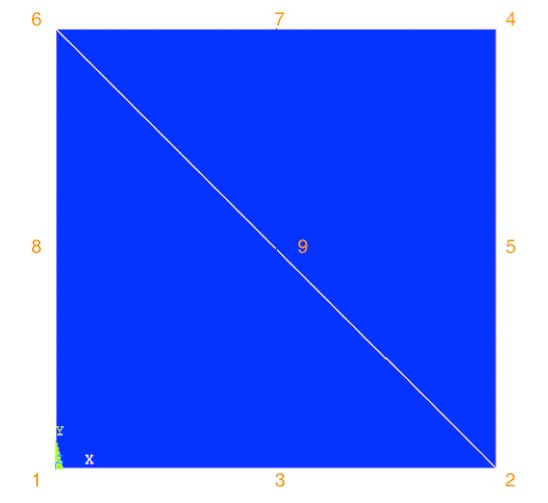
\includegraphics[width=6cm,clip]{muster.png} 			
		\caption{A simple meshed geometry} \label{fig: muster}
	\end{center}
\end{figure}

\begin{table}
	\begin{center}
		\caption{Node list exported from ANSYS}\label{tab: node_list}
		\begin{tabular}{ ccccccc }
			\hline			
			NODE & X & Y & Z & THXY & THYZ & THZX\\ \hline
			1 & 0.0000 & 0.0000 & 0.0000 & 0.00 & 0.00 & 0.00 \\
			2 & 50.000 & 0.0000 & 0.0000 & 0.00 & 0.00 & 0.00 \\
			3 & 25.000 & 0.0000 & 0.0000 & 0.00 & 0.00 & 0.00 \\
			4 & 50.000 & 50.000 & 0.0000 & 0.00 & 0.00 & 0.00 \\
			5 & 50.000 & 25.000 & 0.0000 & 0.00 & 0.00 & 0.00 \\
			6 & 0.0000 & 50.000 & 0.0000 & 0.00 & 0.00 & 0.00 \\
			7 & 25.000 & 50.000 & 0.0000 & 0.00 & 0.00 & 0.00 \\
			8 & 0.0000 & 25.000 & 0.0000 & 0.00 & 0.00 & 0.00 \\
			9 & 25.000 & 25.000 & 0.0000 & 0.00 & 0.00 & 0.00 \\
			\hline  
		\end{tabular}	
	\end{center}
\end{table}

\begin{table}
	\begin{center}
		\caption{Element list exported from ANSYS}\label{tab: element_list}
		\begin{tabular}{ cccccccccccc }
			\hline			
			ELEM & MAT & TYP & REL & ESY & SEC & Node & Node  & Node & Node & Node & Node\\ \hline
			1 & 1 & 1 & 1 & 0 & 1 & 6 & 2 & 4 & 9 & 5 & 7 \\
			2 & 1 & 1 & 1 & 0 & 1 & 6 & 1 & 2 & 8 & 3 & 9 \\
			\hline  
		\end{tabular}		
	\end{center}	
\end{table}

\chapter{Element Type Test}
\section{Unit Testing with Python}
According to the documentation of Fred L. Drake, Jr. [\cite{Python}], automated unit testing is the best way to determine whether the element type works well. Unit test is the batteries-included test module in the Python standard library. The motivation for writing a unit testing is to evaluate the quality of each element type and try to find the reasons for failed tests. The element types to be tested are Tri3, Tri6, Quad4, Quad8, Tet4 and Tet10. We test the strain and stress components with all the element types. As is mentioned before, the numerical solution to a mechanical problem is only an approximate solution. There is an error between the analytical solution and FEM solution for sure. Here we do not have an analytical solution to compare with our AMfe solution. The components from ANSYS will be compared to the results that are calculated from AMfe Toolbox. Although the solution from ANSYS is not the analytical solution, it could still help us check the quality of element types in AMfe Toolbox. As a comparison, we need to define both the absolute error and the relative error in the test. According to the work of Rao V. Dukkipati [\cite{NumericalMethod}], absolute error is the magnitude of the difference between actual value and approximate value. It can be defined as:
\begin{equation}
e_{abs} = \|X_{actual} - X_{fem} \|
\end{equation}
Relative error is the absolute error relative to the actual value. It can be defined as:
\begin{equation}
e_{rel} = \frac{\|X_{actual} - X_{fem} \|}{X_{actual}}
\end{equation} 
As Rao V. Dukkipati [\cite{NumericalMethod}] has noted, "it is noteworthy that errors of approximation or rounding and truncation are introduced by numerical methods or algorithms and calculating with finite precision. Truncation error represents the error that occurs when some series is truncated to a fewer number of terms. Such error is virtually an algorithmic error. Roundoff error occurs because of the computing tool's inability to handle certain numbers." It is hard to set one tolerance standard for all engineering problems. The tolerance for error can vary in different situations. One thing we can do here is set the tolerance with different values and compare the results of testing between elements. 
In the engineering field, Von Mises stress is usually regarded as a failure criterion to judge a design. Hence, here we calculate the von Mises stress by meshing with each element type in their corresponding 2D or 3D models. According to the research of P. M. Kurowski [\cite{VonMiese}], the Von Mises stress can be expressed by the principle stresses as:
\begin{equation}
\sigma_{vm} = \sqrt{\frac{1}{2}\left[\left(\sigma_1 - \sigma_2\right)^2 + \left(\sigma_2 - \sigma_3\right)^2 + \left(\sigma_3 - \sigma_1\right)^2\right]}
\end{equation}
The 2D and 3D model for unit testing are build in a simple way. We create a rectangle for 2D elements and a cube for 3D elements. We apply only Dirichlet boundary condition on these models. Figure \ref{fig: PatchMuster} and Figure \ref{fig: UnitTest3D} illustrate the model for 2D and 3D element, respectively. 
The complete test of all the element types is shown in Table \ref{tab: DirectTesting} and Table \ref{tab: SRTesting}. It is obvious that both algorithms perform well in Tri3 and Quad4. The other element types fail the unit test. It is necessary to investigate into what is wrong with the other element types. 

\begin{figure}
	\begin{center}
		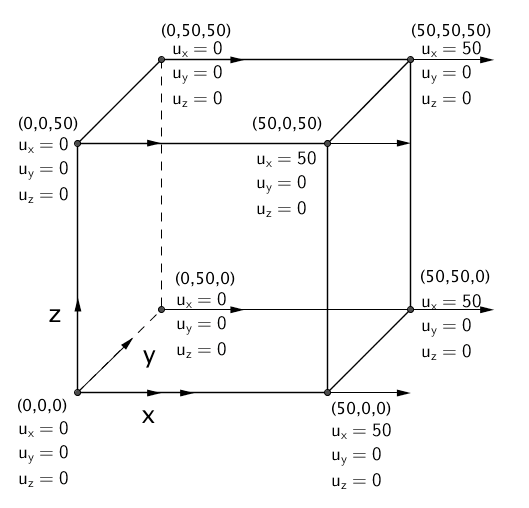
\includegraphics[width=6cm,clip]{UnitTest3D.png} 			
		\caption{A model for test of 3D elements} \label{fig: UnitTest3D}
	\end{center}
\end{figure}

\begin{table} 		
	\caption{Unit testing of the result using Direct-Evaluation-Algorithms}
	\label{tab: DirectTesting}
\begin{tabular}{l*{5}{c}r} 

	Tolerance Parameter              & Tri3 & Tri6 & Quad4 & Quad8 & Tet4  & Tet10  \\
	\hline
	$e_{abs}=10^{-10}$; $e_{rel}=10^{-4}$ & Fail & Fail & Fail & Fail & Fail & Fail   \\
	$e_{abs}=10^{-10}$; $e_{rel}=5\times10^{-4}$&  Pass& Fail & Fail & Fail & Fail &  Fail  \\
	$e_{abs}=10^{-10}$; $e_{rel}=10^{-3}$ & Pass & Fail & Pass & Fail &  Fail & Fail   \\
   \hline
\end{tabular}
\end{table}

\begin{table} 		
	\caption{Unit testing of the extrapolate result using Stress-Recovery-Algorithms}
	\label{tab: SRTesting}
	\begin{tabular}{l*{5}{c}r} 
		
		Tolerance Parameter    & Tri3 & Tri6 & Quad4 & Quad8 & Tet4  & Tet10  \\
		\hline
		$e_{abs}=10^{-10}$; $e_{rel}=10^{-4}$ & Fail & Fail & Fail & Fail & Fail & Fail   \\
		$e_{abs}=10^{-10}$; $e_{rel}=5\times10^{-4}$&  Pass& Fail & Fail & Fail & Fail &  Fail  \\
		$e_{abs}=10^{-10}$; $e_{rel}=10^{-3}$ & Pass & Fail & Pass & Fail &  Fail & Fail   \\
		\hline
	\end{tabular}
\end{table}

\section{The Patch Test}
After testing the quality of each element type, we find out that the element types Tri6, Quad8, Tet4, and Tet10 are problematic and need to fixed. In order to fix these problems, we need to know if the finite element program has the correct algorithmic procedure. This is generally not easy to verify when the modelling is too complex. The patch test is a useful technique in checking the performance of element type that is being tested. The basic idea of the patch test is to apply special boundary conditions so as to maintain a constant strain and a constant stress field. This is to simplify a complex problem to a simple one, to which we already know the correct numerical solutions. \\
According to the theory of Carlos A. Felippa [\cite{Felippa} section 15 p.9-11], the procedures of the displacement patch test are as follows: create a simple geometry that consists of one or several element; pick a patch and apply the displacement at exterior nodes and the prescribed displacement field will be set as $u_x = x, u_y = 0$. The reason the displacement field only applies to exterior nodes is that displacements are related to the background continuum. The last step is to verify whether the patch has a constant strain field. The mechanism behind the displacement patch test is setting the strain at every exterior node as 1, which is can be calculated by:
\begin{equation}
\frac{\mathrm d u}{\mathrm d x} = 1
\end{equation}
As we know, 
\begin{equation}
\sum N_i = 1
\end{equation}
and, 
\begin{equation}
\epsilon = \sum N_i \cdot \epsilon_{i}
\end{equation}
Here we have $\epsilon_i = 0$ and $\sum N_i = 1$, hence the strain field is constant and equal 1. \\
Now we take Tri3 as an example in implementing the displacement patch test. We create a simple rectangle that consists of two Tri3 element in ANSYS, and the prescribed displacement field is depicted in Figure \ref{fig: PatchMuster}. Strain field from ANSYS can be viewed in Figure \ref{fig: PatchTest}. As is expected, $\epsilon_{xx} = 1$. Thus, we have successfully built the model for a patch test. Now it is time to check whether AMfe Toolbox has the same constant strain field or not. We export the node, element, and displacement data from ANSYS and import all of them into AMfe Toolbox. After computing strain and strtess in AMfe, the contour plot of strain in ParaView is shown as the picture on right-hand side of Figure \ref{fig: PatchTest}. The plot from AMfe Toolbox illustrates the same result of $\epsilon_ {xx} = 1$. This proves that the displacement patch test has been passed. Other element types,  namely Tri6, Quad4, Quad8, Tet4, and Tet10, each have a constant field. However, the results of the patch test using element Tri6, Quad8, Tet4, and Tet10 are still problematic because all of these elements have the value of 1.5 as the constant strain, as is demonstrate by the problematic result from Tet4 in Figure \ref{fig: Tet4Patch}. It is necessary to investigate why all these elements have the same strain with the value of 1.5.  By debugging the AMfe Code we can find that the strain values at Gauss points are all 1.5. This proves that the Stress-Recovery-Algorithms is correct. The problem exists in the calculation of the strain at Gauss points. Moreover, all of these element types except Tri3 and Quad4 have the same problem.   

\begin{figure}
	\begin{center}
		\includegraphics[width=10cm,clip]{PatchMuster.pdf} 			
		\caption{A model for test of 2D elements} \label{fig: PatchMuster}
	\end{center}
\end{figure}

\begin{figure}
	\begin{center}
		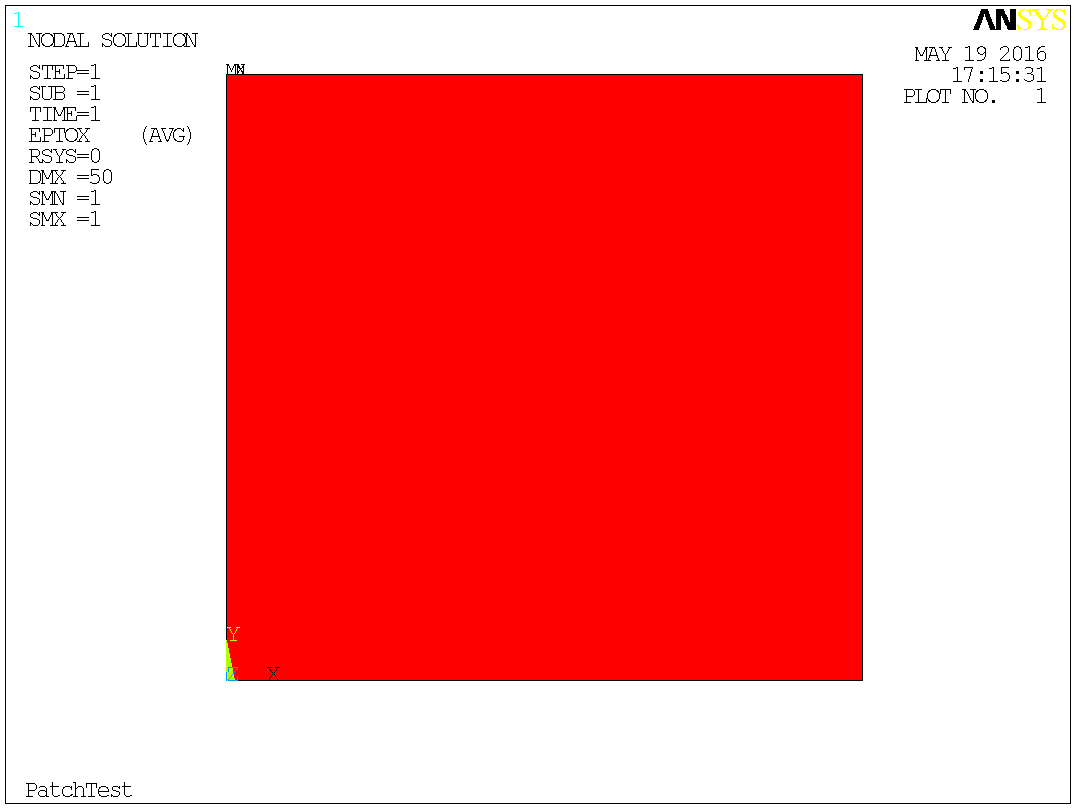
\includegraphics[width=6cm,clip]{PatchTest.png} 		
		\includegraphics[width=7cm,clip]{PatchParaView.pdf} 		
		\caption{left: Contour plot of $\epsilon_{xx}$ from ANSYS (SMN: minimal value; SMX: maximal value); right: Contour plot of $\epsilon_{xx}$ calculated in AMfe, demonstrate in ParaView} \label{fig: PatchTest}
	\end{center}
\end{figure}

\begin{figure}
	\begin{center}
		\includegraphics[width=8cm,clip]{Tet4Patch.pdf} 			
		\caption{Patch Test of Tet4} \label{fig: Tet4Patch}
	\end{center}
\end{figure}

\section{Convergence Analysis}
We can either decrease the element size or increase the polynomial degrees of the shape function to approach an relatively exact approximation. This process is denoted as convergence. A convergence analysis provides a function to reduce the relative error of the solution with increasing number of degrees of freedom [\cite{FiniteElement}]. An example of convergence analysis is illustrated in Figure \ref{fig: convergence}. On the one hand, because of the technical restriction, we can only export the node, element, and displacement lists from ANSYS and set all of them as input into AMfe Toolbox for solving strain and stress. As of now, we did not reverse the process and solve the displacement by using prescribed Neumann boundary condition and Dirichlet boundary condition as input. However, it is still a feasible plan for future research. On the other hand, we can analyse this problem using another software, Gmsh, as Pre-Processing tool. The procedures of our convergence analysis for investigating 2D elements are as follows: first, we create a 2D geometry in ANSYS and generate a fine meshing with element types Quad4, Quad8, Tri3, and Tri6, respectively. Then we pick one node to view the displacement. In this case, we do not have the analytical solution, thus the displacement result in this fine meshing will be regarded as a referential solution. In next step, we create an identical modelling in Gmsh and refine the meshing of all the 2D element types by decreasing the size of the elements. Then, we can record the displacement results of both AMfe and ANSYS from meshing with different degrees of freedom (DOFs), and plot the corresponding ratios of AMfe results to ANSYS results. The 3D element types, Tet4 and Tet10, can also be analysed using this approach. An example of 2D model meshing with Tri3 is shown in Figure \ref{fig: Convergence2D} and an example of 3D model meshing with Tet4 is shown in Figure \ref{fig: Convergence3D}.
The displacement for each of the 2D element types has been recorded in Table \ref{tab: TriConvergence} and Table \ref{tab: QuadConvergence}. The displacement for 3D element types are represented in Table \ref{tab: TetConvergence}. The same nodal displacements from a fine meshing in ANSYS are:
\begin{equation*}
2D: Ux = -0.0015045; Uy = 0.011738
\end{equation*}

\begin{equation*}
3D: Ux = 9.47; Uy = 0; Uz = 0
\end{equation*}
The convergence plots of 2D element types are depicted in Figure \ref{fig: TriConPlot} and Figure \ref{fig: QuadConPlot}. Figure \ref{fig: TetConPlot} shows the convergence performance of 3D element types. All the element types show a good convergence to the exact solution. The higher order element types (Tri6 and Tet10) have a relatively higher convergence rate than the lower order element types (Tri3 and Tet4) do. This characteristic is not that discernible in quadrilateral element types (Quad4 and Quad8). 

\begin{figure}[htbp]
	\begin{center}	
		\includegraphics[width=9cm,clip]{convergence.pdf} 			
		\caption{Convergence analysis} \label{fig: convergence}
	\end{center}
\end{figure}


\begin{figure}[htbp]
	\begin{center}	
		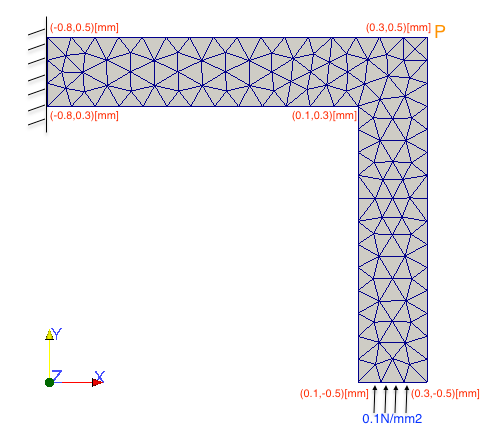
\includegraphics[width=10cm,clip]{Convergence2D.png} 			
		\caption{2D model meshing with Tri3 for displacement convergence analysis; P as observer point} \label{fig: Convergence2D}
	\end{center}
\end{figure}

\begin{figure}[htbp]
	\begin{center}	
		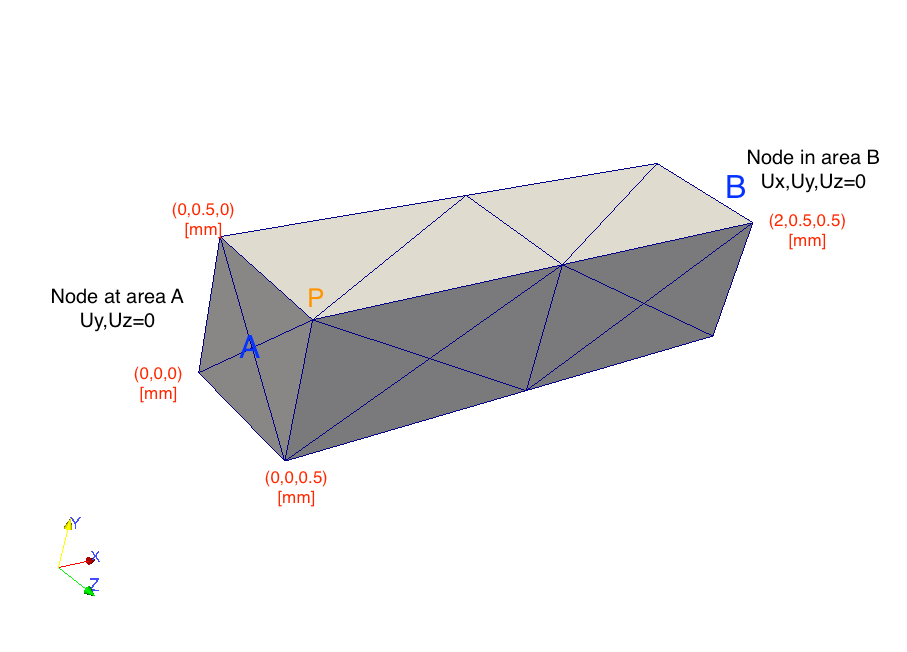
\includegraphics[width=14cm,clip]{Convergence3D.png} 			
		\caption{3D model meshing with Tet4 for displacement convergence analysis; P as observer point} \label{fig: Convergence3D}
	\end{center}
\end{figure}

\begin{figure}[htbp]
	\begin{center}	
		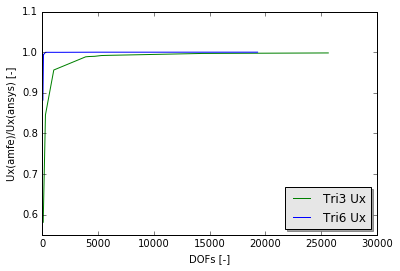
\includegraphics[width=7cm,clip]{TriConPlotUx.png}
		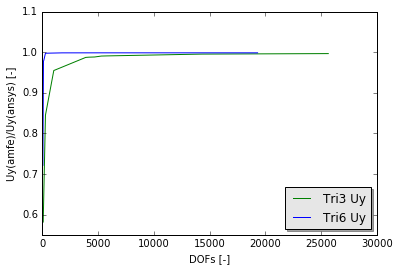
\includegraphics[width=7cm,clip]{TriConPlotUy.png} 	 			
		\caption{Convergence plot of Tri3 and Tri6} \label{fig: TriConPlot}
	\end{center}
\end{figure}

\begin{figure}[htbp]
	\begin{center}	
		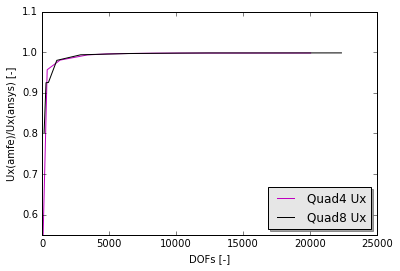
\includegraphics[width=7cm,clip]{QuadConPlotUx.png}
		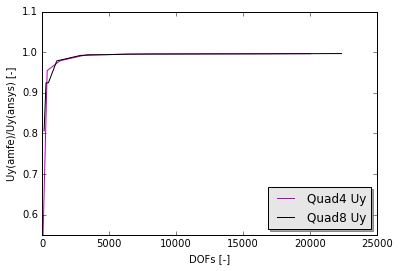
\includegraphics[width=7cm,clip]{QuadConPlotUy.png} 	 			
		\caption{Convergence plot of Quad4 and Quad8} \label{fig: QuadConPlot}
	\end{center}
\end{figure}

\begin{figure}[htbp]
	\begin{center}	
		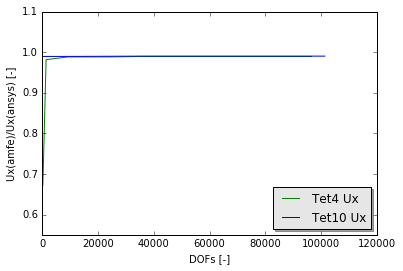
\includegraphics[width=9cm,clip]{TetConPlotUx.png}	 			
		\caption{Convergence plot of Tet4 and Tet10} \label{fig: TetConPlot}
	\end{center}
\end{figure}

\begin{table}[ht]
		\caption{Convergence analysis of displacement for triangular element}
		\label{tab: TriConvergence}
\begin{tabular}{ c | c | c | c | c | c} 	
	DOFs & Tri3-Ux & Tri3-Uy & DOFs &Tri6-Ux & Tri6-Uy\\ \hline
	90 & -0.000873929 & 0.0068367 & 62 & -0.00132675 & 0.00847992  \\ 
	292 & -0.00127231 & 0.00993406 & 114 & -0.00149616 & 0.011506 \\
	1038 & -0.00143843 & 0.0112263 & 138 & -0.00149623 & 0.011513  \\
	3898 & -0.00148735 &  0.0112263&  292 & -0.001504 & 0.0117277 \\
	4170 & -0.00148835 &  0.0116131&  1780 & -0.001504 & 0.0117383\\
	4698 & -0.00148919 &  0.0116189& 4830 & -0.00150448 & 0.0117391  \\
	5298 & -0.00149204 &  0.0116457& 8986 & -0.00150449 & 0.0117392 \\
	5842 & -0.00149269 &  0.0116505&  12073 & -0.00150450 & 0.0117392\\
	14322 & -0.00149982 & 0.0117028& 15609 & -0.00150451 & 0.0117393 \\
	25634 & -0.00150168 & 0.0117171 & 19300 &  -0.00150453 &  0.0117393\\
	\hline  
\end{tabular}
\end{table}


\begin{table}[ht]
	\caption{Convergence analysis of displacement for quadrilateral element} \label{tab: QuadConvergence}
	\begin{tabular}{ c | c | c | c | c | c} 	
		DOFs & Quad4-Ux & Quad4-Uy & DOFs &Quad8-Ux & Quad8-Uy\\ \hline
		48 & -0.00078276 & 0.00620667 & 142 & -0.00120593 & 0.00847992  \\ 
		372 & -0.0014393 & 0.0112254 & 286 & -0.00139123& 0.0108697 \\
		1332 & -0.00147509 & 0.0115086 & 466 & -0.00139228 & 0.0108725  \\
		3374 & -0.00149431 &  0.0116894&  1090 & -0.00147418& 0.0115056 \\
		4842 & -0.00149817 &  0.0116894&  2870 &-0.00149483 & 0.0116652\\
		6228 & -0.00149945 &  0.0116992& 6450 &  -0.00149948 & 0.0117018  \\
		8386 & -0.00150076 &   0.0117105& 10346 &  -0.00150103 & 0.0117032 \\
		10232 & -0.00150123 &  0.0117123&  12342 & -0.00150163 & 0.0117056\\
		15344 &-0.00150134 & 0.0117144& 15656 & -0.00150166 & 0.0117079 \\
		20044 & -0.00150143 & 0.0117151 & 22344 &  -0.00150183 &  0.0117186\\
		\hline  
	\end{tabular}
\end{table}

\begin{table}[ht]
	\caption{Convergence analysis of displacement for tetrahedral element} \label{tab: TetConvergence}
	\begin{tabular}{ c | c | c | c | c | c | c | c} 	
		DOFs & Tet4-Ux & Tet4-Uy & Tet4-Uz & DOFs & Tet10-Ux & Tet10-Uy & Tet10-Uz\\ \hline
		54 & 6.320 & 0 & 0 & 243 & 9.370& 0  & 0 \\ 
		243 & 6.372 & 0 & 0 & 579 & 9.370&0 & 0\\
		1395 & 9.295 & 0 & 0 & 13857 & 9.372&  0 & 0 \\
		9315 & 9.360 &  0 &  0 & 36312&9.378 &0 & 0\\
		24579 & 9.360 &  0 &  0 & 43521 & 9.378&0 & 0\\
		34632 & 9.370 &  0 & 0 &  57537 & 9.378&0 & 0  \\
		53307 & 9.370 &   0 & 0 &  60299 & 9.378&0 & 0 \\
		64343 & 9.370 & 0 &  0 & 79683 & 9.378&0 & 0\\
		76443 & 9.370 & 0 & 0 & 84322 & 9.378 &0 & 0 \\
		96567 & 9.370 & 0 & 0 &  101321 & 9.378& 0& 0\\
		\hline  
	\end{tabular}
\end{table}
It is also important to check the convergence of Von Mises stress. Thus we refine the meshing in a 2D or 3D modelling using all the element types in ANSYS, and then export the data of node, element, and displacement from ANSYS and import them into AMfe Toolbox. The next step is to run the code to get the computing results for our convergence study. $\sigma_{xy}$, $\sigma_{yy}$, $\sigma_{zz}$ are for 2D convergence analysis and $\sigma_{xy}$, $\sigma_{yy}$, $\sigma_{zz}$, $\sigma_{xy}$, $\sigma_{yz}$, $\sigma_{xz}$ are for 3D convergence analysis.   Then we can use these values to calculate the Von Mises stress: 
\begin{equation}
\sigma_v = \sqrt{\frac{1}{2}\left[\left(\sigma_{11}-\sigma_{22}\right)^2 + \left(\sigma_{22}-\sigma_{33}\right)^2 + \left(\sigma_{33}-\sigma_{11}\right)^2 + 6\left({\sigma_{12}}^2 + {\sigma_{23}}^2 + {\sigma_{31}}^2 \right) \right]}
\end{equation}
For a general plane stress case with restrictions $\sigma_3 = 0$, $\sigma_{31} = \sigma_{23} = 0$, we can simplify the Von Mises equation as:
\begin{equation}
\sigma_v = \sqrt{{\sigma_{11}}^2 - \sigma_{11}\sigma_{22} + {\sigma_{22}}^2 + 3 {\sigma_{12}}^2}
\end{equation}
The 2D model is built as shown in Figure \ref{fig: twoDmodel} and the 3D model is built as shown in Figure \ref{fig: threeDmodel}. Table \ref{tab: 2DConvergence} shows the test data of convergence analysis for all element types. Figure \ref{fig: ConPlot} illustrate the relation between the DOFs of mesh and the Von Mises stress of the observer point, which is denoted C in 2D model and is denoted D in 3D model. The three plots in Figure \ref{fig: ConPlot} show that all the element types converges to the exact solution and the elements with higher order (Tri6, Quad8, and Tet10) converges faster than the the one with lower order (Tri3, Quad4, and Tet4). When we compare the two 2D element Tri3 and Quad4, we can find the Quad4 has a higher convergence rate than Tri3. 

\begin{figure}[htbp]
	\begin{center}	
		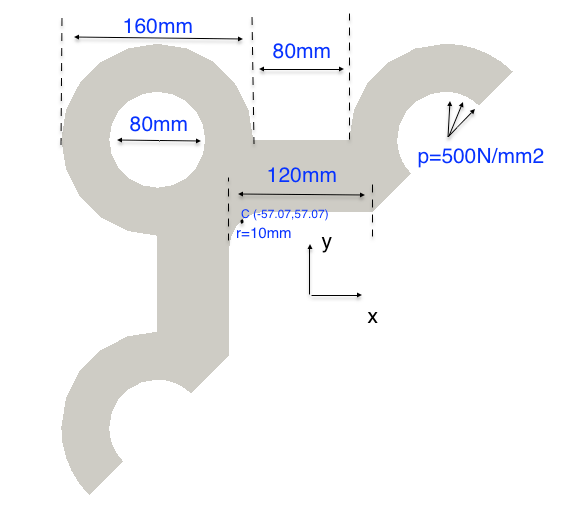
\includegraphics[width=9cm,clip]{twoDmodel.png} 			
		\caption{Convergence analysis of Von Mises stress in a 2D model} \label{fig: twoDmodel}
	\end{center}
\end{figure}

\begin{figure}[htbp]
	\begin{center}	
		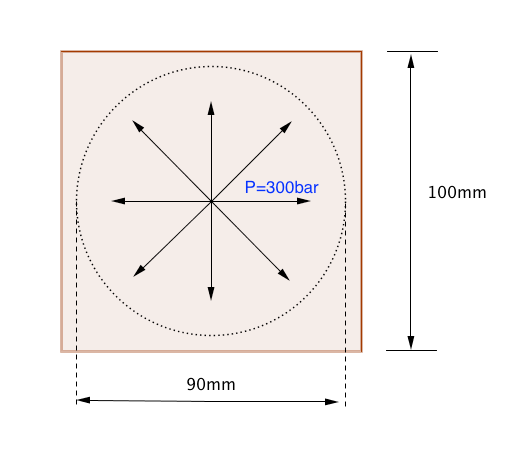
\includegraphics[width=7cm,clip]{threeDmodel1.png} 
	    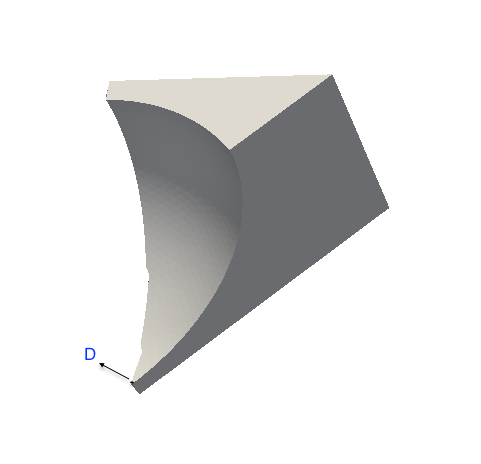
\includegraphics[width=7cm,clip]{threeDmodel2.png} 			
		\caption{Left: Top view of the tank; Right: the 1/16 model of the tank, point D is regarded as the observer point for analysis} \label{fig: threeDmodel}
	\end{center}
\end{figure}

\begin{table}[ht]
	\caption{Convergence analysis of Von Mises stress} \label{tab: 2DConvergence}
	\begin{tabular}{ c | c | c | c | c | c | c | c | c| c |c |c } 	
		DOFs & Tri3 & DOFs & Tri6 & DOFs & Quad4 & DOFs & Quad8 &DOFs&Tet4&DOFs&Tet10 \\ \hline
		870 & 1812.47 & 3132 & 2106.11 & 854 & 1979.22& 2372  & 2109.74 &1101&90.07&588&71.33 \\ 
		2682 & 1952.20 & 10058 & 2127.91 & 2320 & 2074.70&6314 & 2126.62&1725 & 86.24 & 906 & 70.41\\
		4172 & 1981.88 & 15892 &2130.58 & 3448 & 2096.34&  9890 & 2129.87& 3039 & 73.73 & 1352 & 69.53\\
		5788 & 2009.47 &  22286 &2133.51 & 4882& 2104.64 &13648 & 2135.88&4440 & 72.34 &  2258 &  69.39\\
		9354 & 2030.88 &  36028 &2138.76 & 7856 & 2112.48&18340 & 2134.44&5652 & 70.57 &  3396 & 69.21\\
		10952 & 2039.58 &  42344 &2139.34&  9128 & 2113.38&22036 & 2136.23 &6366 & 70.21 &  4351 & 69.16 \\
		15490 & 2055.98 &   49044 &2137.02&  12310 & 2118.76&25724 & 2137.70& 10461 & 69.52 & 5243 & 69.13\\
		27332 & 2073.44 & 60214 &2136.87& 21060 & 2122.70&35096 & 2134.58 & 12342& 69.87& 11721&  69.13\\
		33770 &  2082.39& - & -  & 26384&2127.35&-&-&-&-&-&-\\
		45032 & 2106.63 & - & - & 29056&2128.73&-&-&-&-&-&-\\
		68943 & 2124.15 & - & - &  32548& 2128.16&-&-&-&-&-&-\\
		- & - & - & - &  36750& 2128.62&-&-&-&-&-&-\\
		\hline  
	\end{tabular}
\end{table}


\begin{figure}[htbp]
	\begin{center}	
		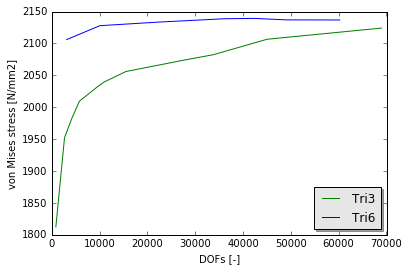
\includegraphics[width=7cm,clip]{triCon.png} 
		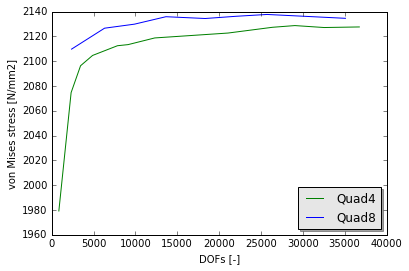
\includegraphics[width=7cm,clip]{quadCon.png} 	
        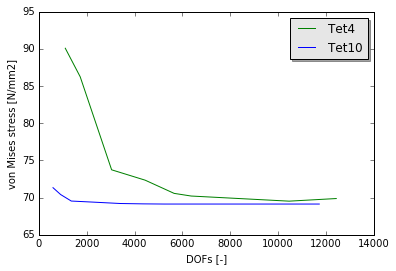
\includegraphics[width=7cm,clip]{tetCon.png} 			
		\caption{Convergence analysis of Von Mises stress, the analytical solutions are 2147.43$N/mm^2$ for 2D model and 68.94$N/mm^2$ for 3D model} \label{fig: ConPlot}
	\end{center}
\end{figure}


\section{Complex Model Test}
The patch test is only applicable to the simple models, it is meaningful how these element type behave in a complex model. Now we create a relatively complex model meshing with each element type and calculate in AMfe by both algorithm, namely, direct evaluation at nodes and extrapolation from Gauss points, namely, Stress-Recovery-Algorithms. The main objective of complex model test is to compare the strain and stress contour plot of each element type in ANSYS and in AMfe Toolbox with both algorithm. Furthermore, the comparison between the two algorithm is also significant for our research. The results from AMfe Toolbox display in ParaView as a Post-Processing tool. It is worth noting that the order of components for tensors follows this mapping rule: 0-xx; 1-yy; 2-zz;  3-yy; 4-yz; 5-xz; 6-zz; 7-xz; 8-xy. For a clear comparison and good contrast, we import a same color map for ANSYS and ParaView. However, there exists still a clear chromatic aberration between the contour plots from ANSYS and ParaView. Figure \ref{fig: QuadConPlot} shows an example to display the color difference. This issue may be fixed when we using an advanced ANSYS version, because ANSYS 12.0, which we use in this paper, can only offers a 7-bit color in color map. 

Figure \ref{fig: Tri3_Exx} to Figure \ref{fig: Tri3_Sxy} illustrate the contour plot of strain and stress in all direction. The contour plots from AMfe are meshed with element type Tri3 and the contour plot from ANSYS is meshed with element PLANE42(triangular option). According to the documentation of ANSYS [\cite{APDL}], "PLANE42 is used for 2D modeling of solid structures. The element can be used either as a plane element (plane stress or plane strain) or as an axisymmetric element. The element is defined by four nodes having two degrees of freedom at each node: translations in the nodal $x$ and $y$ directions."
From the comparison we can find that there is no difference between the both algorithm in AMfe. The results of all components are very similar to the ANSYS solution. 

Figure \ref{fig: Tri6_Exx} to Figure \ref{fig: Tri6_Sxy} illustrate the contour plot of strain and stress in all direction. The contour plots from AMfe are meshed with element type Tri6 and the contour plot from ANSYS is meshed with element PLANE2. According to the documentation of ANSYS [\cite{APDL}], "PLANE2 is a 6-node triangular element. The element is defined by six nodes having two degrees of freedom at each node: translations in the nodal $x$ and $y$ directions." The plots show that the solution with Stress-Recovery-Algorithms is relative close to the ANSYS solution, the algorithm without Stress-Recovery-Algorithm has a higher strain and stress than ANSYS solution at corner points and the inner side of circle. 

Figure \ref{fig: Quad4_Exx} to Figure \ref{fig: Quad4_Sxy} illustrate the contour plot of strain and stress in all direction. The contour plots from AMfe are meshed with element type Quad4 and the contour plot from ANSYS is meshed with element PLANE42 (quadrangle option). We can observe from the plots that the solution by Stress-Recovery-Algorithms is close to ANSYS solution. The deviation of results of the both algorithms appear at some position as it shown in Plots with Tri6.  

Figure \ref{fig: Quad8_Exx} to Figure \ref{fig: Quad8_Sxy} illustrate the contour plot of strain and stress in all direction. The contour plots from AMfe are meshed with element type Quad8 and the contour plot from ANSYS is meshed with element PLANE82. According to the documentation of ANSYS [\cite{APDL}], "Plane82 is a higher order version of the 2D, four node element (PLANE82). It provides more accurate results for mixed (quadrilateral-triangular) automatic meshes and can tolerate irregular shapes without as much loss of accuracy. The 8-node element is defined by eight nodes having two degrees of freedom at each node: translations in nodal $x$ and $y$ directions." The comparison is similar as the result, which is meshed with Quad4. 

Figure \ref{fig: Tet4_Exx} to Figure \ref{fig: Tet4_Sxy} illustrate the contour plot of strain and stress in all direction. The contour plots from AMfe are meshed with element type Tet4 and the contour plot from ANSYS is meshed with element SOLID45. According to the documentation of ANSYS [\cite{APDL}], "SOLID45 is used for the 3D modeling of solid structures. The element is defined by eight nodes having three degrees of freedom at each node: translations in the nodal $x$, $y$, and $z$ directions." The plots represents that there is no difference between the both algorithm in AMfe. The both solution of AMfe have a relative bad performance in shear strain/stress than normal strain/stress. 

Figure \ref{fig: Tet10_Exx} to Figure \ref{fig: Tet10_Sxy} illustrate the contour plot of strain and stress in all direction. The contour plots from AMfe are meshed with element type Tet10 and the contour plot from ANSYS is meshed with element SOLID187 (tetrahedron option). According to the documentation of ANSYS [\cite{APDL}], "SOLID187 element is a higher order 3D, 10-node element. SOLID187 has a quadratic displacement behavior and is well suited to modeling irregular meshes. The element is defined by 10 nodes having three degrees of freedom at each node: translations in the nodal $x$, $y$, and $z$ directions." Tet10 has a same problem as Tet4, the solutions in shear components appear not good. The plots also show that the solutions with Stress-Recovery-Algorithms has a better performance than the solutions  without Stress-Recovery-Algorithm. 

\begin{figure}
	\begin{center}
		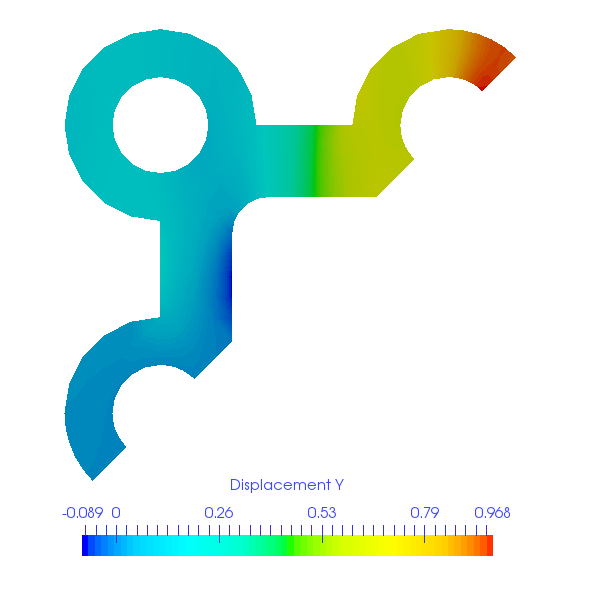
\includegraphics[width=5.5cm,clip]{ParaViewColor.png} 	
		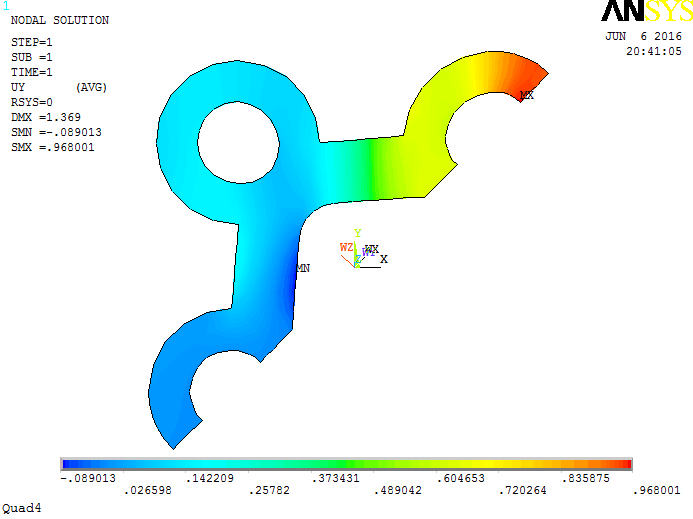
\includegraphics[width=7cm,clip]{ANSYSColor.png} 	
		\caption{Chromatic aberration between ParaView and ANSYS} \label{fig: Color}
	\end{center}
\end{figure}
\clearpage 

\begin{figure}[htbp]
	\begin{center}
		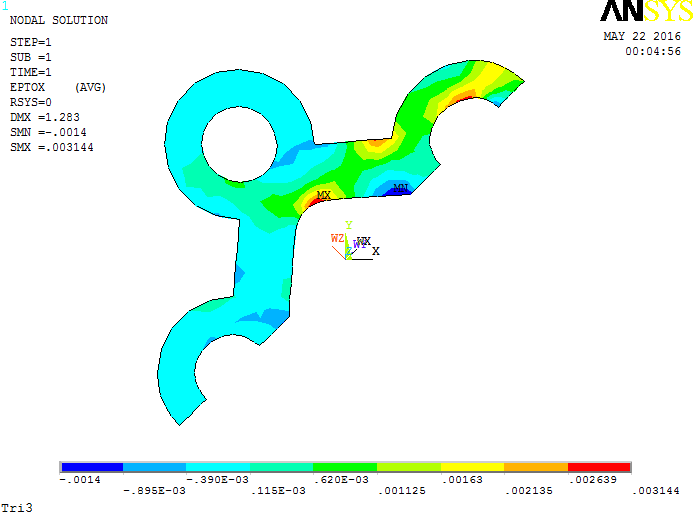
\includegraphics[width=11cm,clip]{TTri3_Exx.png} 	
		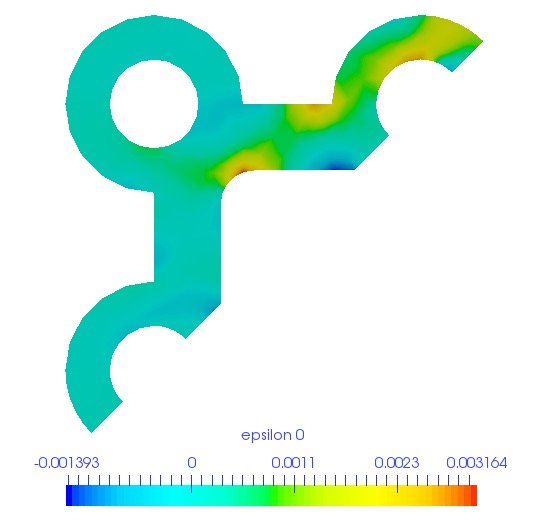
\includegraphics[width=7cm,clip]{TTri3_Exx_PD.png} 	
		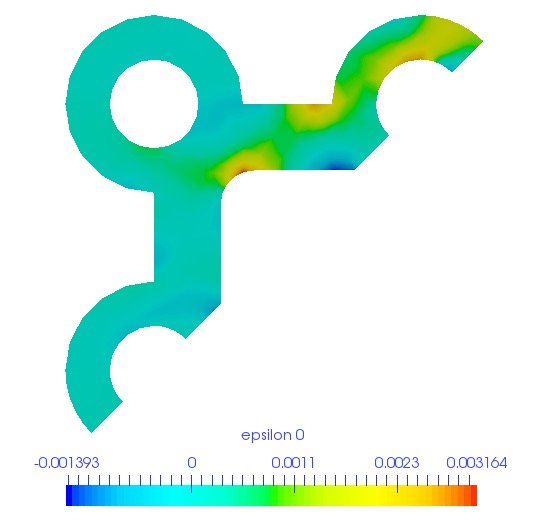
\includegraphics[width=7cm,clip]{TTri3_Exx_P.png} 	
		\caption{Mesh with Tri3, upper: contour plot of $\epsilon_{xx}$ in ANSYS; lower left: contour plot of $\epsilon_{xx}$ calculated without stress recovery in AMfe; lower right: contour plot of $\epsilon_{xx}$ calculated with stress recovery in AMfe} \label{fig: Tri3_Exx}
	\end{center}
\end{figure}
\clearpage 

\begin{figure}[htbp]
	\begin{center}
		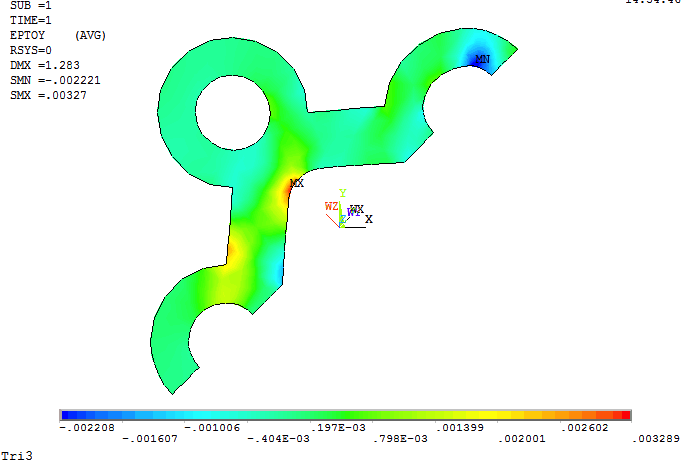
\includegraphics[width=11cm,clip]{TTri3_Eyy.png} 	
		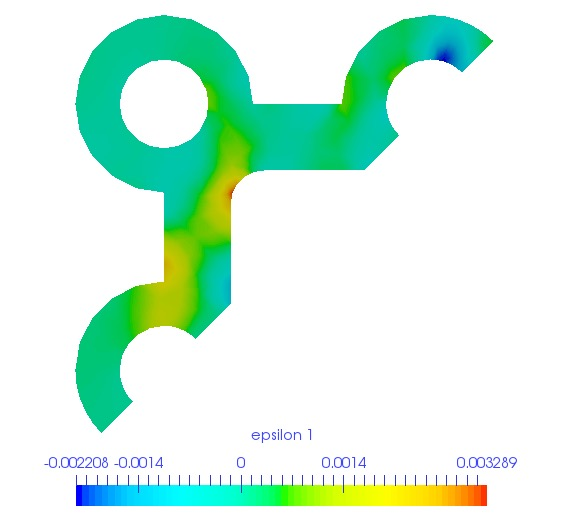
\includegraphics[width=7cm,clip]{TTri3_Eyy_PD.png} 	
		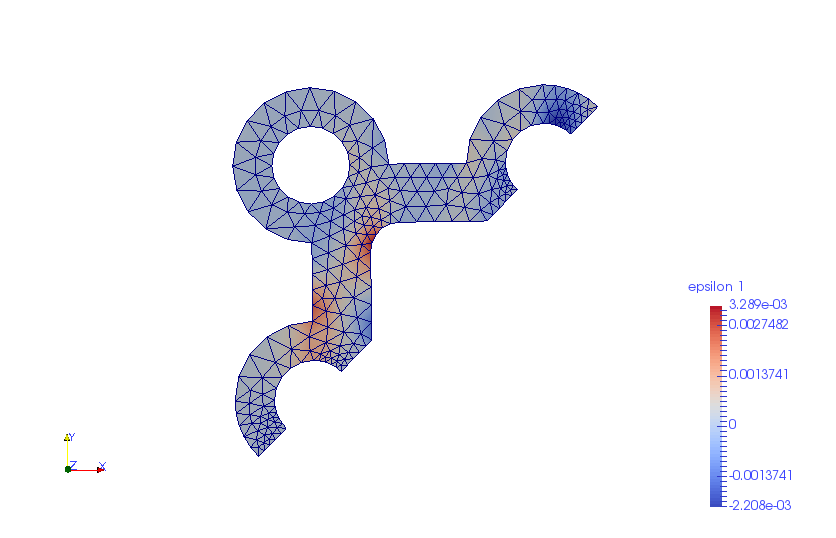
\includegraphics[width=7cm,clip]{TTri3_Eyy_P.png} 		
		\caption{Mesh with Tri3, upper: contour plot of $\epsilon_{yy}$ in ANSYS; lower left: contour plot of $\epsilon_{yy}$ calculated without stress recovery in AMfe; lower right: contour plot of $\epsilon_{yy}$ calculated with stress recovery in AMfe} \label{fig: Tri3_Eyy}
	\end{center}
\end{figure}
\clearpage 

\begin{figure}[htbp]
	\begin{center}
		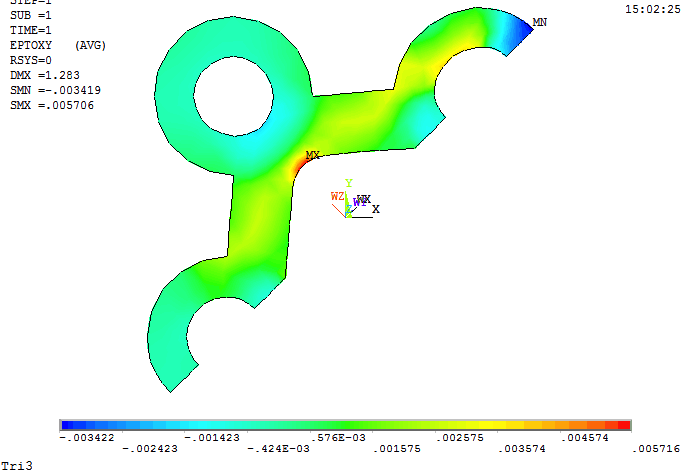
\includegraphics[width=11cm,clip]{TTri3_Exy.png} 
		\includegraphics[width=7cm,clip]{TTri3_Exy_PD.png} 		
		\includegraphics[width=7cm,clip]{TTri3_Exy_P.png} 		
		\caption{Mesh with Tri3, upper: contour plot of $\epsilon_{xy}$ in ANSYS; lower left: contour plot of $\epsilon_{xy}$ calculated without stress recovery in AMfe; lower right: contour plot of $\epsilon_{xy}$ calculated with stress recovery in AMfe} \label{fig: Tri3_Exy}
	\end{center}
\end{figure}
\clearpage 

\begin{figure}[htbp]
	\begin{center}
		\includegraphics[width=11cm,clip]{TTri3_Sxx.png} 	
		\includegraphics[width=7cm,clip]{TTri3_Sxx_PD.png} 		
		\includegraphics[width=7cm,clip]{TTri3_Sxx_P.png} 		
		\caption{Mesh with Tri3, upper: contour plot of $\sigma_{xx}$ in ANSYS; lower left: contour plot of $\sigma_{xx}$ calculated without stress recovery in AMfe; lower right: contour plot of $\sigma_{xx}$ calculated with stress recovery in AMfe} \label{fig: Tri3_Sxx}
	\end{center}
\end{figure}
\clearpage 

\begin{figure}[htbp]
	\begin{center}
		\includegraphics[width=11cm,clip]{TTri3_Syy.png} 	
		\includegraphics[width=7cm,clip]{TTri3_Syy_PD.png} 	
		\includegraphics[width=7cm,clip]{TTri3_Syy_P.png} 		
		\caption{Mesh with Tri3, upper: contour plot of $\sigma_{yy}$ in ANSYS; lower left: contour plot of $\sigma_{yy}$ calculated without stress recovery in AMfe; lower right: contour plot of $\sigma_{yy}$ calculated with stress recovery in AMfe} \label{fig: Tri3_Syy}
	\end{center}
\end{figure}
\clearpage 

\begin{figure}[htbp]
	\begin{center}
		\includegraphics[width=11cm,clip]{TTri3_Sxy.png} 	
		\includegraphics[width=7cm,clip]{TTri3_Sxy_PD.png} 		
		\includegraphics[width=7cm,clip]{TTri3_Sxy_P.png} 		
		\caption{Mesh with Tri3, upper: contour plot of $\sigma_{xy}$ in ANSYS; lower left: contour plot of $\sigma_{xy}$ calculated without stress recovery in AMfe; lower right: contour plot of $\sigma_{xy}$ calculated with stress recovery in AMfe} \label{fig: Tri3_Sxy}
	\end{center}
\end{figure}
\clearpage 

\begin{figure}[htbp]
	\begin{center}
		\includegraphics[width=11cm,clip]{Tri6_Exx.png} 	
		\includegraphics[width=7cm,clip]{Tri6_Exx_PD.png} 		
		\includegraphics[width=7cm,clip]{Tri6_Exx_P.png} 		
		\caption{Mesh with Tri6, upper: contour plot of $\epsilon_{xx}$ in ANSYS; lower left: contour plot of $\epsilon_{xx}$ calculated without stress recovery in AMfe; lower right: contour plot of $\epsilon_{xx}$ calculated with stress recovery in AMfe} \label{fig: Tri6_Exx}
	\end{center}
\end{figure}
\clearpage 

\begin{figure}[htbp]
	\begin{center}
		\includegraphics[width=11cm,clip]{Tri6_Eyy.png} 
		\includegraphics[width=7cm,clip]{Tri6_Eyy_PD.png} 		
		\includegraphics[width=7cm,clip]{Tri6_Eyy_P.png} 		
		\caption{Mesh with Tri6, upper: contour plot of $\epsilon_{yy}$ in ANSYS; lower left: contour plot of $\epsilon_{yy}$ calculated without stress recovery in AMfe; lower right: contour plot of $\epsilon_{yy}$ calculated with stress recovery in AMfe} \label{fig: Tri6_Eyy}
	\end{center}
\end{figure}
\clearpage 

\begin{figure}[htbp]
	\begin{center}
		\includegraphics[width=11cm,clip]{Tri6_Exy.png} 	
		\includegraphics[width=7cm,clip]{Tri6_Exy_PD.png} 	
		\includegraphics[width=7cm,clip]{Tri6_Exy_P.png} 		
		\caption{Mesh with Tri6, upper: contour plot of $\epsilon_{xy}$ in ANSYS; lower left: contour plot of $\epsilon_{xy}$ calculated without stress recovery in AMfe; lower right: contour plot of $\epsilon_{xy}$ calculated with stress recovery in AMfe} \label{fig: Tri6_Exy}
	\end{center}
\end{figure}
\clearpage 

\begin{figure}[htbp]
	\begin{center}
		\includegraphics[width=11cm,clip]{Tri6_Sxx.png} 	
		\includegraphics[width=7cm,clip]{Tri6_Sxx_PD.png} 	
		\includegraphics[width=7cm,clip]{Tri6_Sxx_P.png} 		
		\caption{Mesh with Tri6, upper: contour plot of $\sigma_{xx}$ in ANSYS; lower left: contour plot of $\sigma_{xx}$ calculated without stress recovery in AMfe; lower right: contour plot of $\sigma_{xx}$ calculated with stress recovery in AMfe} \label{fig: Tri6_Sxx}
	\end{center}
\end{figure}
\clearpage 

\begin{figure}[htbp]
	\begin{center}
		\includegraphics[width=11cm,clip]{Tri6_Syy.png} 	
		\includegraphics[width=7cm,clip]{Tri6_Syy_PD.png} 		
		\includegraphics[width=7cm,clip]{Tri6_Syy_P.png} 		
		\caption{Mesh with Tri6, upper: contour plot of $\sigma_{yy}$ in ANSYS; lower left: contour plot of $\sigma_{yy}$ calculated without stress recovery in AMfe; lower right: contour plot of $\sigma_{yy}$ calculated with stress recovery in AMfe} \label{fig: Tri6_Syy}
	\end{center}
\end{figure}
\clearpage 

\begin{figure}[htbp]
	\begin{center}
		\includegraphics[width=11cm,clip]{Tri6_Sxy.png} 		
		\includegraphics[width=7cm,clip]{Tri6_Sxy_PD.png} 		
		\includegraphics[width=7cm,clip]{Tri6_Sxy_P.png} 		
		\caption{Mesh with Tri6, upper: contour plot of $\sigma_{xy}$ in ANSYS; lower left: contour plot of $\sigma_{xy}$ calculated without stress recovery in AMfe; lower right: contour plot of $\sigma_{xy}$ calculated with stress recovery in AMfe} \label{fig: Tri6_Sxy}
	\end{center}
\end{figure}
\clearpage 


\begin{figure}[htbp]
	\begin{center}
		\includegraphics[width=11cm,clip]{Quad4_Exx.png} 
		\includegraphics[width=7cm,clip]{Quad4_Exx_PD.png} 				
		\includegraphics[width=7cm,clip]{Quad4_Exx_P.png} 		
		\caption{Mesh with Quad4, upper: contour plot of $\epsilon_{xx}$ in ANSYS; lower left: contour plot of $\epsilon_{xx}$ calculated without stress recovery in AMfe; lower right: contour plot of $\epsilon_{xx}$ calculated with stress recovery in AMfe} \label{fig: Quad4_Exx}
	\end{center}
\end{figure}
\clearpage 

\begin{figure}[htbp]
	\begin{center}
		\includegraphics[width=11cm,clip]{Quad4_Eyy.png} 	
		\includegraphics[width=7cm,clip]{Quad4_Eyy_PD.png} 		
		\includegraphics[width=7cm,clip]{Quad4_Eyy_P.png} 		
		\caption{Mesh with Quad4, upper: contour plot of $\epsilon_{yy}$ in ANSYS; lower left: contour plot of $\epsilon_{yy}$ calculated without stress recovery in AMfe; lower right: contour plot of $\epsilon_{yy}$ calculated with stress recovery in AMfe} \label{fig: Quad4_Eyy}
	\end{center}
\end{figure}
\clearpage 

\begin{figure}[htbp]
	\begin{center}
		\includegraphics[width=11cm,clip]{Quad4_Exy.png} 	
		\includegraphics[width=7cm,clip]{Quad4_Exy_PD.png} 		
		\includegraphics[width=7cm,clip]{Quad4_Exy_P.png} 		
		\caption{Mesh with Quad4, upper: contour plot of $\epsilon_{xy}$ in ANSYS; lower left: contour plot of $\epsilon_{xy}$ calculated without stress recovery in AMfe; lower right: contour plot of $\epsilon_{xy}$ calculated with stress recovery in AMfe} \label{fig: Quad4_Exy}
	\end{center}
\end{figure}
\clearpage 

\begin{figure}[htbp]
	\begin{center}
		\includegraphics[width=11cm,clip]{Quad4_Sxx.png} 
		\includegraphics[width=7cm,clip]{Quad4_Sxx_PD.png} 			
		\includegraphics[width=7cm,clip]{Quad4_Sxx_P.png} 		
		\caption{Mesh with Quad4, upper: contour plot of $\sigma_{xx}$ in ANSYS; lower left: contour plot of $\sigma_{xx}$ calculated without stress recovery in AMfe; lower right: contour plot of $\sigma_{xx}$ calculated with stress recovery in AMfe} \label{fig: Quad4_Sxx}
	\end{center}
\end{figure}
\clearpage 

\begin{figure}[htbp]
	\begin{center}
		\includegraphics[width=11cm,clip]{Quad4_Syy.png} 
		\includegraphics[width=7cm,clip]{Quad4_Syy_PD.png} 			
		\includegraphics[width=7cm,clip]{Quad4_Syy_P.png} 		
		\caption{Mesh with Quad4, upper: contour plot of $\sigma_{yy}$ in ANSYS; lower left: contour plot of $\sigma_{yy}$ calculated without stress recovery in AMfe; lower right: contour plot of $\sigma_{yy}$ calculated with stress recovery in AMfe} \label{fig: Quad4_Syy}
	\end{center}
\end{figure}
\clearpage 

\begin{figure}[htbp]
	\begin{center}
		\includegraphics[width=11cm,clip]{Quad4_Sxy.png} 	
		\includegraphics[width=7cm,clip]{Quad4_Sxy_PD.png} 	
		\includegraphics[width=7cm,clip]{Quad4_Sxy_P.png} 		
		\caption{Mesh with Quad4, upper: contour plot of $\sigma_{xy}$ in ANSYS; lower left: contour plot of $\sigma_{xy}$ calculated without stress recovery in AMfe; lower right: contour plot of $\sigma_{xy}$ calculated with stress recovery in AMfe} \label{fig: Quad4_Sxy}
	\end{center}
\end{figure}
\clearpage 

\begin{figure}[htbp]
	\begin{center}
		\includegraphics[width=11cm,clip]{Quad8_Exx.png} 	
		\includegraphics[width=7cm,clip]{Quad8_Exx_PD.png} 	
		\includegraphics[width=7cm,clip]{Quad8_Exx_P.png} 		
		\caption{Mesh with Quad8, upper: contour plot of $\epsilon_{xx}$ in ANSYS; lower left: contour plot of $\epsilon_{xx}$ calculated without stress recovery in AMfe; lower right: contour plot of $\epsilon_{xx}$ calculated with stress recovery in AMfe} \label{fig: Quad8_Exx}
	\end{center}
\end{figure}
\clearpage 

\begin{figure}[htbp]
	\begin{center}
		\includegraphics[width=11cm,clip]{Quad8_Eyy.png} 	
		\includegraphics[width=7cm,clip]{Quad8_Eyy_PD.png} 			
		\includegraphics[width=7cm,clip]{Quad8_Eyy_P.png} 		
		\caption{Mesh with Quad8, upper: contour plot of $\epsilon_{yy}$ in ANSYS; lower left: contour plot of $\epsilon_{yy}$ calculated without stress recovery in AMfe; lower right: contour plot of $\epsilon_{yy}$ calculated with stress recovery in AMfe} \label{fig: Quad8_Eyy}
	\end{center}
\end{figure}
\clearpage 

\begin{figure}[htbp]
	\begin{center}
		\includegraphics[width=11cm,clip]{Quad8_Exy.png} 
		\includegraphics[width=7cm,clip]{Quad8_Exy_PD.png} 			
		\includegraphics[width=7cm,clip]{Quad8_Exy_P.png} 		
		\caption{Mesh with Quad8, upper: contour plot of $\epsilon_{xy}$ in ANSYS; lower left: contour plot of $\epsilon_{xy}$ calculated without stress recovery in AMfe; lower right: contour plot of $\epsilon_{xy}$ calculated with stress recovery in AMfe} \label{fig: Quad8_Exy}
	\end{center}
\end{figure}
\clearpage 

\begin{figure}[htbp]
	\begin{center}
		\includegraphics[width=11cm,clip]{Quad8_Sxx.png} 
		\includegraphics[width=7cm,clip]{Quad8_Sxx_PD.png} 			
		\includegraphics[width=7cm,clip]{Quad8_Sxx_P.png} 		
		\caption{Mesh with Quad8, upper: contour plot of $\sigma_{xx}$ in ANSYS; lower left: contour plot of $\sigma_{xx}$ calculated without stress recovery in AMfe; lower right: contour plot of $\sigma_{xx}$ calculated with stress recovery in AMfe} \label{fig: Quad8_Sxx}
	\end{center}
\end{figure}
\clearpage 

\begin{figure}[htbp]
	\begin{center}
		\includegraphics[width=11cm,clip]{Quad8_Syy.png} 	
		\includegraphics[width=7cm,clip]{Quad8_Syy_PD.png} 		
		\includegraphics[width=7cm,clip]{Quad8_Syy_P.png} 		
		\caption{Mesh with Quad8, upper: contour plot of $\sigma_{yy}$ in ANSYS; lower left: contour plot of $\sigma_{yy}$ calculated without stress recovery in AMfe; lower right: contour plot of $\sigma_{yy}$ calculated with stress recovery in AMfe} \label{fig: Quad8_Syy}
	\end{center}
\end{figure}
\clearpage 

\begin{figure}[htbp]
	\begin{center}
		\includegraphics[width=11cm,clip]{Quad8_Sxy.png} 
		\includegraphics[width=7cm,clip]{Quad8_Sxy_PD.png} 		
		\includegraphics[width=7cm,clip]{Quad8_Sxy_P.png} 		
		\caption{Mesh with Quad8, upper: contour plot of $\sigma_{xy}$ in ANSYS; lower left: contour plot of $\sigma_{xy}$ calculated without stress recovery in AMfe; lower right: contour plot of $\sigma_{xy}$ calculated with stress recovery in AMfe} \label{fig: Quad8_Sxy}
	\end{center}
\end{figure}
\clearpage 

\begin{figure}[htbp]
	\begin{center}
		\includegraphics[width=13cm,clip]{Tet4Exx.png} 	
		\includegraphics[width=7cm,clip]{Tet4ExxPD.png} 			
		\includegraphics[width=7cm,clip]{Tet4ExxP.png} 		
		\caption{Mesh with Tet4, upper: contour plot of $\epsilon_{xx}$ in ANSYS; lower left: contour plot of $\epsilon_{xx}$ calculated without stress recovery in AMfe; lower right: contour plot of $\epsilon_{xx}$ calculated with stress recovery in AMfe} \label{fig: Tet4_Exx}
	\end{center}
\end{figure}
\clearpage 

\begin{figure}[htbp]
	\begin{center}
		\includegraphics[width=13cm,clip]{Tet4Eyy.png} 		
		\includegraphics[width=7cm,clip]{Tet4EyyPD.png} 
		\includegraphics[width=7cm,clip]{Tet4EyyP.png} 		
		\caption{Mesh with Tet4, upper: contour plot of $\epsilon_{yy}$ in ANSYS; lower left: contour plot of $\epsilon_{yy}$ calculated without stress recovery in AMfe; lower right: contour plot of $\epsilon_{yy}$ calculated with stress recovery in AMfe} \label{fig: Tet4_Eyy}
	\end{center}
\end{figure}
\clearpage 

\begin{figure}[htbp]
	\begin{center}
		\includegraphics[width=13cm,clip]{Tet4Ezz.png} 
		\includegraphics[width=7cm,clip]{Tet4EzzPD.png} 				
		\includegraphics[width=7cm,clip]{Tet4EzzP.png} 		
		\caption{Mesh with Tet4, upper: contour plot of $\epsilon_{zz}$ in ANSYS; lower left: contour plot of $\epsilon_{zz}$ calculated without stress recovery in AMfe; lower right: contour plot of $\epsilon_{zz}$ calculated with stress recovery in AMfe} \label{fig: Tet4_Ezz}
	\end{center}
\end{figure}
\clearpage 

\begin{figure}[htbp]
	\begin{center}
		\includegraphics[width=13cm,clip]{Tet4Exy.png} 	
		\includegraphics[width=7cm,clip]{Tet4ExyPD.png} 			
		\includegraphics[width=7cm,clip]{Tet4ExyP.png} 		
		\caption{Mesh with Tet4, upper: contour plot of $\epsilon_{xy}$ in ANSYS; lower left: contour plot of $\epsilon_{xy}$ calculated without stress recovery in AMfe; lower right: contour plot of $\epsilon_{xy}$ calculated with stress recovery in AMfe} \label{fig: Tet4_Exy}
	\end{center}
\end{figure}
\clearpage 

\begin{figure}[htbp]
	\begin{center}
		\includegraphics[width=13cm,clip]{Tet4Eyz.png} 	
		\includegraphics[width=7cm,clip]{Tet4EyzPD.png} 			
		\includegraphics[width=7cm,clip]{Tet4EyzP.png} 		
		\caption{Mesh with Tet4, upper: contour plot of $\epsilon_{yz}$ in ANSYS; lower left: contour plot of $\epsilon_{yz}$ calculated without stress recovery in AMfe; lower right: contour plot of $\epsilon_{yz}$ calculated with stress recovery in AMfe} \label{fig: Tet4_Eyz}
	\end{center}
\end{figure}
\clearpage 

\begin{figure}[htbp]
	\begin{center}
		\includegraphics[width=13cm,clip]{Tet4Exz.png} 	
		\includegraphics[width=7cm,clip]{Tet4ExzPD.png} 	
		\includegraphics[width=7cm,clip]{Tet4ExzP.png} 		
		\caption{Mesh with Tet4, upper: contour plot of $\epsilon_{xz}$ in ANSYS; lower left: contour plot of $\epsilon_{xz}$ calculated without stress recovery in AMfe; lower right: contour plot of $\epsilon_{xz}$ calculated with stress recovery in AMfe} \label{fig: Tet4_Exz}
	\end{center}
\end{figure}
\clearpage 

\begin{figure}[htbp]
	\begin{center}
		\includegraphics[width=13cm,clip]{Tet4Sxx.png} 	
		\includegraphics[width=7cm,clip]{Tet4SxxPD.png} 	
		\includegraphics[width=7cm,clip]{Tet4SxxP.png} 		
		\caption{Mesh with Tet4, upper: contour plot of $\sigma_{xx}$ in ANSYS; lower left: contour plot of $\sigma_{xx}$ calculated without stress recovery in AMfe; lower right: contour plot of $\sigma_{xx}$ calculated with stress recovery in AMfe} \label{fig: Tet4_Sxx}
	\end{center}
\end{figure}
\clearpage 

\begin{figure}[htbp]
	\begin{center}
		\includegraphics[width=13cm,clip]{Tet4Syy.png} 
		\includegraphics[width=7cm,clip]{Tet4SyyPD.png} 			
		\includegraphics[width=7cm,clip]{Tet4SyyP.png} 		
		\caption{Mesh with Tet4, upper: contour plot of $\sigma_{yy}$ in ANSYS; lower left: contour plot of $\sigma_{yy}$ calculated without stress recovery in AMfe; lower right: contour plot of $\sigma_{yy}$ calculated with stress recovery in AMfe} \label{fig: Tet4_Syy}
	\end{center}
\end{figure}
\clearpage 

\begin{figure}[htbp]
	\begin{center}
		\includegraphics[width=13cm,clip]{Tet4Szz.png} 	
		\includegraphics[width=7cm,clip]{Tet4SzzPD.png} 	
		\includegraphics[width=7cm,clip]{Tet4SzzP.png} 		
		\caption{Mesh with Tet4, upper: contour plot of $\sigma_{zz}$ in ANSYS; lower left: contour plot of $\sigma_{zz}$ calculated without stress recovery in AMfe; lower right: contour plot of $\sigma_{zz}$ calculated with stress recovery in AMfe} \label{fig: Tet4_Szz}
	\end{center}
\end{figure}
\clearpage 

\begin{figure}[htbp]
	\begin{center}
		\includegraphics[width=13cm,clip]{Tet4Sxy.png} 		
		\includegraphics[width=7cm,clip]{Tet4SxyPD.png} 	
		\includegraphics[width=7cm,clip]{Tet4SxyP.png} 		
		\caption{Mesh with Tet4, upper: contour plot of $\sigma_{xy}$ in ANSYS; lower left: contour plot of $\sigma_{xy}$ calculated without stress recovery in AMfe; lower right: contour plot of $\sigma_{xy}$ calculated with stress recovery in AMfe} \label{fig: Tet4_Sxy}
	\end{center}
\end{figure}
\clearpage 

\begin{figure}[htbp]
	\begin{center}
		\includegraphics[width=13cm,clip]{Tet4Syz.png} 
		\includegraphics[width=7cm,clip]{Tet4SyzPD.png} 			
		\includegraphics[width=7cm,clip]{Tet4SyzP.png} 		
		\caption{Mesh with Tet4, upper: contour plot of $\sigma_{yz}$ in ANSYS; lower left: contour plot of $\sigma_{yz}$ calculated without stress recovery in AMfe; lower right: contour plot of $\sigma_{yz}$ calculated with stress recovery in AMfe} \label{fig: Tet4_Syz}
	\end{center}
\end{figure}
\clearpage 

\begin{figure}[htbp]
	\begin{center}
		\includegraphics[width=13cm,clip]{Tet4Sxz.png} 
		\includegraphics[width=7cm,clip]{Tet4SxzPD.png} 		
		\includegraphics[width=7cm,clip]{Tet4SxzP.png} 		
		\caption{Mesh with Tet4, upper: contour plot of $\sigma_{xz}$ in ANSYS; lower left: contour plot of $\sigma_{xz}$ calculated without stress recovery in AMfe; lower right: contour plot of $\sigma_{xz}$ calculated with stress recovery in AMfe} \label{fig: Tet4_Sxz}
	\end{center}
\end{figure}
\clearpage 

\begin{figure}[htbp]
	\begin{center}
		\includegraphics[width=11cm,clip]{Tet10_Exx.png}
		\includegraphics[width=7cm,clip]{Tet10_Exx_PD.png}  		
		\includegraphics[width=7cm,clip]{Tet10_Exx_P.png} 		
		\caption{Mesh with Tet10, upper: contour plot of $\epsilon_{xx}$ in ANSYS; lower left: contour plot of $\epsilon_{xx}$ calculated without stress recovery in AMfe; lower right: contour plot of $\epsilon_{xx}$ calculated with stress recovery in AMfe} \label{fig: Tet10_Exx}
	\end{center}
\end{figure}
\clearpage 

\begin{figure}[htbp]
	\begin{center}
		\includegraphics[width=11cm,clip]{Tet10_Eyy.png} 	
		\includegraphics[width=7.5cm,clip]{Tet10_Eyy_PD.png} 		
		\includegraphics[width=7cm,clip]{Tet10_Eyy_P.png} 		
		\caption{Mesh with Tet10, upper: contour plot of $\epsilon_{yy}$ in ANSYS; lower left: contour plot of $\epsilon_{yy}$ calculated without stress recovery in AMfe; lower right: contour plot of $\epsilon_{yy}$ calculated with stress recovery in AMfe} \label{fig: Tet10_Eyy}
	\end{center}
\end{figure}
\clearpage 

\begin{figure}[htbp]
	\begin{center}
		\includegraphics[width=11cm,clip]{Tet10_Ezz.png} 
		\includegraphics[width=7.5cm,clip]{Tet10_Ezz_PD.png} 		
		\includegraphics[width=7cm,clip]{Tet10_Ezz_P.png} 		
		\caption{Mesh with Tet10, upper: contour plot of $\epsilon_{zz}$ in ANSYS; lower left: contour plot of $\epsilon_{zz}$ calculated without stress recovery in AMfe; lower right: contour plot of $\epsilon_{zz}$ calculated with stress recovery in AMfe} \label{fig: Tet10_Ezz}
	\end{center}
\end{figure}
\clearpage 

\begin{figure}[htbp]
	\begin{center}
		\includegraphics[width=11cm,clip]{Tet10_Exy.png} 	
		\includegraphics[width=7cm,clip]{Tet10_Exy_PD.png} 		
		\includegraphics[width=7cm,clip]{Tet10_Exy_P.png} 		
		\caption{Mesh with Tet10, upper: contour plot of $\epsilon_{xy}$ in ANSYS; lower left: contour plot of $\epsilon_{xy}$ calculated without stress recovery in AMfe; lower right: contour plot of $\epsilon_{xy}$ calculated with stress recovery in AMfe} \label{fig: Tet10_Exy}
	\end{center}
\end{figure}
\clearpage 

\begin{figure}[htbp]
	\begin{center}
		\includegraphics[width=11cm,clip]{Tet10_Eyz.png} 	
		\includegraphics[width=7cm,clip]{Tet10_Eyz_PD.png} 	
		\includegraphics[width=7cm,clip]{Tet10_Eyz_P.png} 		
		\caption{Mesh with Tet10, upper: contour plot of $\epsilon_{yz}$ in ANSYS; lower left: contour plot of $\epsilon_{yz}$ calculated without stress recovery in AMfe; lower right: contour plot of $\epsilon_{yz}$ calculated with stress recovery in AMfe} \label{fig: Tet10_Eyz}
	\end{center}
\end{figure}
\clearpage 

\begin{figure}[htbp]
	\begin{center}
		\includegraphics[width=11cm,clip]{Tet10_Exz.png} 
		\includegraphics[width=7cm,clip]{Tet10_Exz_PD.png} 			
		\includegraphics[width=7cm,clip]{Tet10_Exz_P.png} 		
		\caption{Mesh with Tet10, upper: contour plot of $\epsilon_{xz}$ in ANSYS; lower left: contour plot of $\epsilon_{xz}$ calculated without stress recovery in AMfe; lower right: contour plot of $\epsilon_{xz}$ calculated with stress recovery in AMfe} \label{fig: Tet10_Exz}
	\end{center}
\end{figure}
\clearpage 

\begin{figure}[htbp]
	\begin{center}
		\includegraphics[width=11cm,clip]{Tet10_Sxx.png} 	
		\includegraphics[width=7cm,clip]{Tet10_Sxx_PD.png} 			
		\includegraphics[width=7cm,clip]{Tet10_Sxx_P.png} 		
		\caption{Mesh with Tet10, upper: contour plot of $\sigma_{xx}$ in ANSYS; lower left: contour plot of $\sigma_{xx}$ calculated without stress recovery in AMfe; lower right: contour plot of $\sigma_{xx}$ calculated with stress recovery in AMfe} \label{fig: Tet10_Sxx}
	\end{center}
\end{figure}
\clearpage 

\begin{figure}[htbp]
	\begin{center}
		\includegraphics[width=11cm,clip]{Tet10_Syy.png} 	
		\includegraphics[width=7cm,clip]{Tet10_Syy_PD.png} 			
		\includegraphics[width=7cm,clip]{Tet10_Syy_P.png} 		
		\caption{Mesh with Tet10, upper: contour plot of $\sigma_{yy}$ in ANSYS; lower left: contour plot of $\sigma_{yy}$ calculated without stress recovery in AMfe; lower right: contour plot of $\sigma_{yy}$ calculated with stress recovery in AMfe} \label{fig: Tet10_Syy}
	\end{center}
\end{figure}
\clearpage 

\begin{figure}[htbp]
	\begin{center}
		\includegraphics[width=11cm,clip]{Tet10_Szz.png} 
		\includegraphics[width=7cm,clip]{Tet10_Szz_PD.png} 		
		\includegraphics[width=7cm,clip]{Tet10_Szz_P.png} 		
		\caption{Mesh with Tet10, upper: contour plot of $\sigma_{zz}$ in ANSYS; lower left: contour plot of $\sigma_{zz}$ calculated without stress recovery in AMfe; lower right: contour plot of $\sigma_{zz}$ calculated with stress recovery in AMfe} \label{fig: Tet10_Szz}
	\end{center}
\end{figure}
\clearpage 

\begin{figure}[htbp]
	\begin{center}
		\includegraphics[width=11cm,clip]{Tet10_Sxy.png} 	
		\includegraphics[width=7cm,clip]{Tet10_Sxy_PD.png} 		
		\includegraphics[width=7cm,clip]{Tet10_Sxy_P.png} 		
		\caption{Mesh with Tet10, upper: contour plot of $\sigma_{xy}$ in ANSYS; lower left: contour plot of $\sigma_{xy}$ calculated without stress recovery in AMfe; lower right: contour plot of $\sigma_{xy}$ calculated with stress recovery in AMfe} \label{fig: Tet10_Sxy}
	\end{center}
\end{figure}
\clearpage 

\begin{figure}[htbp]
	\begin{center}
		\includegraphics[width=11cm,clip]{Tet10_Syz.png} 		
		\includegraphics[width=7cm,clip]{Tet10_Syz_PD.png} 		
		\includegraphics[width=7cm,clip]{Tet10_Syz_P.png} 		
		\caption{Mesh with Tet10, upper: contour plot of $\sigma_{yz}$ in ANSYS; lower left: contour plot of $\sigma_{yz}$ calculated without stress recovery in AMfe; lower right: contour plot of $\sigma_{yz}$ calculated with stress recovery in AMfe} \label{fig: Tet10_Syz}
	\end{center}
\end{figure}
\clearpage 

\begin{figure}[htbp]
	\begin{center}
		\includegraphics[width=11cm,clip]{Tet10_Sxz.png} 		
		\includegraphics[width=7cm,clip]{Tet10_Sxz_PD.png} 	
		\includegraphics[width=7cm,clip]{Tet10_Sxz_P.png} 		
		\caption{Mesh with Tet10, upper: contour plot of $\sigma_{xz}$ in ANSYS; lower left: contour plot of $\sigma_{xz}$ calculated without stress recovery in AMfe; lower right: contour plot of $\sigma_{xz}$ calculated with stress recovery in AMfe} \label{fig: Tet10_Sxz}
	\end{center}
\end{figure}
\clearpage 

\chapter{Conclusion}
\section{Summary}
There are two algorithms to get the approximation of nodal stress, one is Direct-Evaluation-Algorithms and the other one is Stress-Recovery-Algorithms. The latter one is based on an extrapolation from the Gauss points to the corner nodes. According to different element types, it is necessary to choose the suitable coordinate systems. For quadrilateral elements, the Cartesian coordinate system is appropriate to choose. For triangular and tetrahedral elements, their own coordinate system is more appropriate for the calculation. The type of Gauss element for each element types is also available for selection. We take the selection as follows: 2$\times$2 quadrilateral element with four Gauss points for Quad4; 3$\times$3 quadrilateral element with nine Gauss points for Quad8; triangular element with three Gauss points for Tri3; triangular element with six Gauss points for Tri6; tetrahedral element with four Gauss points for Tet4 and Tet10. The step after extrapolation of stress from Gauss points is to solve the average value at each node by dividing the number of elements that share the same node. And then the nodal stress is finally 'recovered'. 

In the implementation part of this thesis, we export the Pre-Processing data from ANSYS modeling and import into AMfe Toolbox for calculation. Then the solutions by Stress-Recovery-Algorithms and Direct-Evaluation-Algorithms are compared to the ANSYS solution. An unit testing for calculating the Von Mises stress shows that only Tri3 and Quad4 have an acceptable accuracy of Von Mises stress. Thus we do the displacement patch test for each element by the both algorithms. This results of the patch test show that all the element types by both algorithms have passed the patch test and Tri6, Quad8, Tet4, and Tet10 get the constant strain value as 1.5, which expect to 1. And the reason for this issue has been found out by debugging the code. The Pre-calculated strain at Gauss points is 1.5, when the modelling are meshed with Tri6, Quad8, Tet4, and Tet10. Hence the nodal strain after extrapolation is also 1.5. This proves that the Stress-Recovery-Algorithms works well. In addition, the convergence analysis for displacement and Von Mises stress are also checked. The results of displacements convergence analysis represents that all the element types converges to the exact solution. The higher order elements (Tri6 and Tet10) have a relatively higher convergence rate than the lower order elements (Tri3 and Tet4) and this characteristic is not that discernible with quadrilateral elements. The results of Von Mises stress convergence analysis represents that all the element types converges to the exact solution and the elements with higher order (Tri6, Quad8, and Tet10) converges faster than the one with lower order (Tri3, Quad4, and Tet4). The results also show that the Quad4 has a higher convergence rate than Tri3. The last test is to observe the performance of all the element types in a relative complex model. We can not only compare the strain/stress contour plots between the solution by Direct-Evaluation-Algorithms and the solution by Stress-Recovery-Algorithms, but also the strain/stress contour plots between the solution from ANSYS and the solution from AMfe by the both algorithms. The comparison among these three solution express that there is no difference between the solution by the both algorithms for Tri3 and Tet4, and the  solution by Stress-Recovery-Algotithms has a better performance than the solution by Direct-Evaluation-Algorithms for the other element types (Tri6, Quad4, Quad8, and Tet10). The issue by Direct-Evaluation-Algorithms is the deviation at the value around the extreme values, namely the value around maximum and minimum value. The values at the middle part appear rather closer to the ANSYS solution. In summary, Stress-Recovery-Algorithms improves the accuracy of nodal stress for Tri6, Quad4, Quad8, and Tet10 with respect to the Direct-Evaluation-Algorithms.  


\section{Recommendation}
According to the work of Carlos A. Felippa [\cite{Felippa} section 28 p.6], there are two method to calculate the averaged nodal stress after stress recovery. One is the approach, which we apply in this paper, unweighted averaging for the nodal stress. The other one is weighted averaging for the nodal stress, which allocates the weights to the contributions of element sharing the same node. Stress components, element types could affect the weights for selection.

According to the patch test in this paper, we find the issue with the strain at Gauss points with element types Tri6, Quad8, Tet4, and Tet10. Therefore, an investigation for the calculation of strain at Gauss points with these mentioned problematic element types is meaningful to improve the accuracy of nodal strain and stress. 

We discuss in this thesis only about the case of extrapolation from one type of Gauss element. A comparison and discuss of the nodal stress between the extrapolation by using different types of Gauss element would be helpful for the further Stress-Recovery-Algorithms. 

% Testing with all element type and formulate a table
% my_material  = KirchhoffMaterial()	
% 不同单元之间也可以进行比较
\cite{qwe}
\cite{Wang}
\cite{Felippa}\cite{qwe}